\subsection{Further Tests}
\label{furthertests}

In this appendix we describe further tests that we have performed to cross-check the stability and robustness of the $\dnds$ derived in the main text.


\subsubsection{Flat $S^2\,\dnds$}



\begin{figure}[t]
\centering
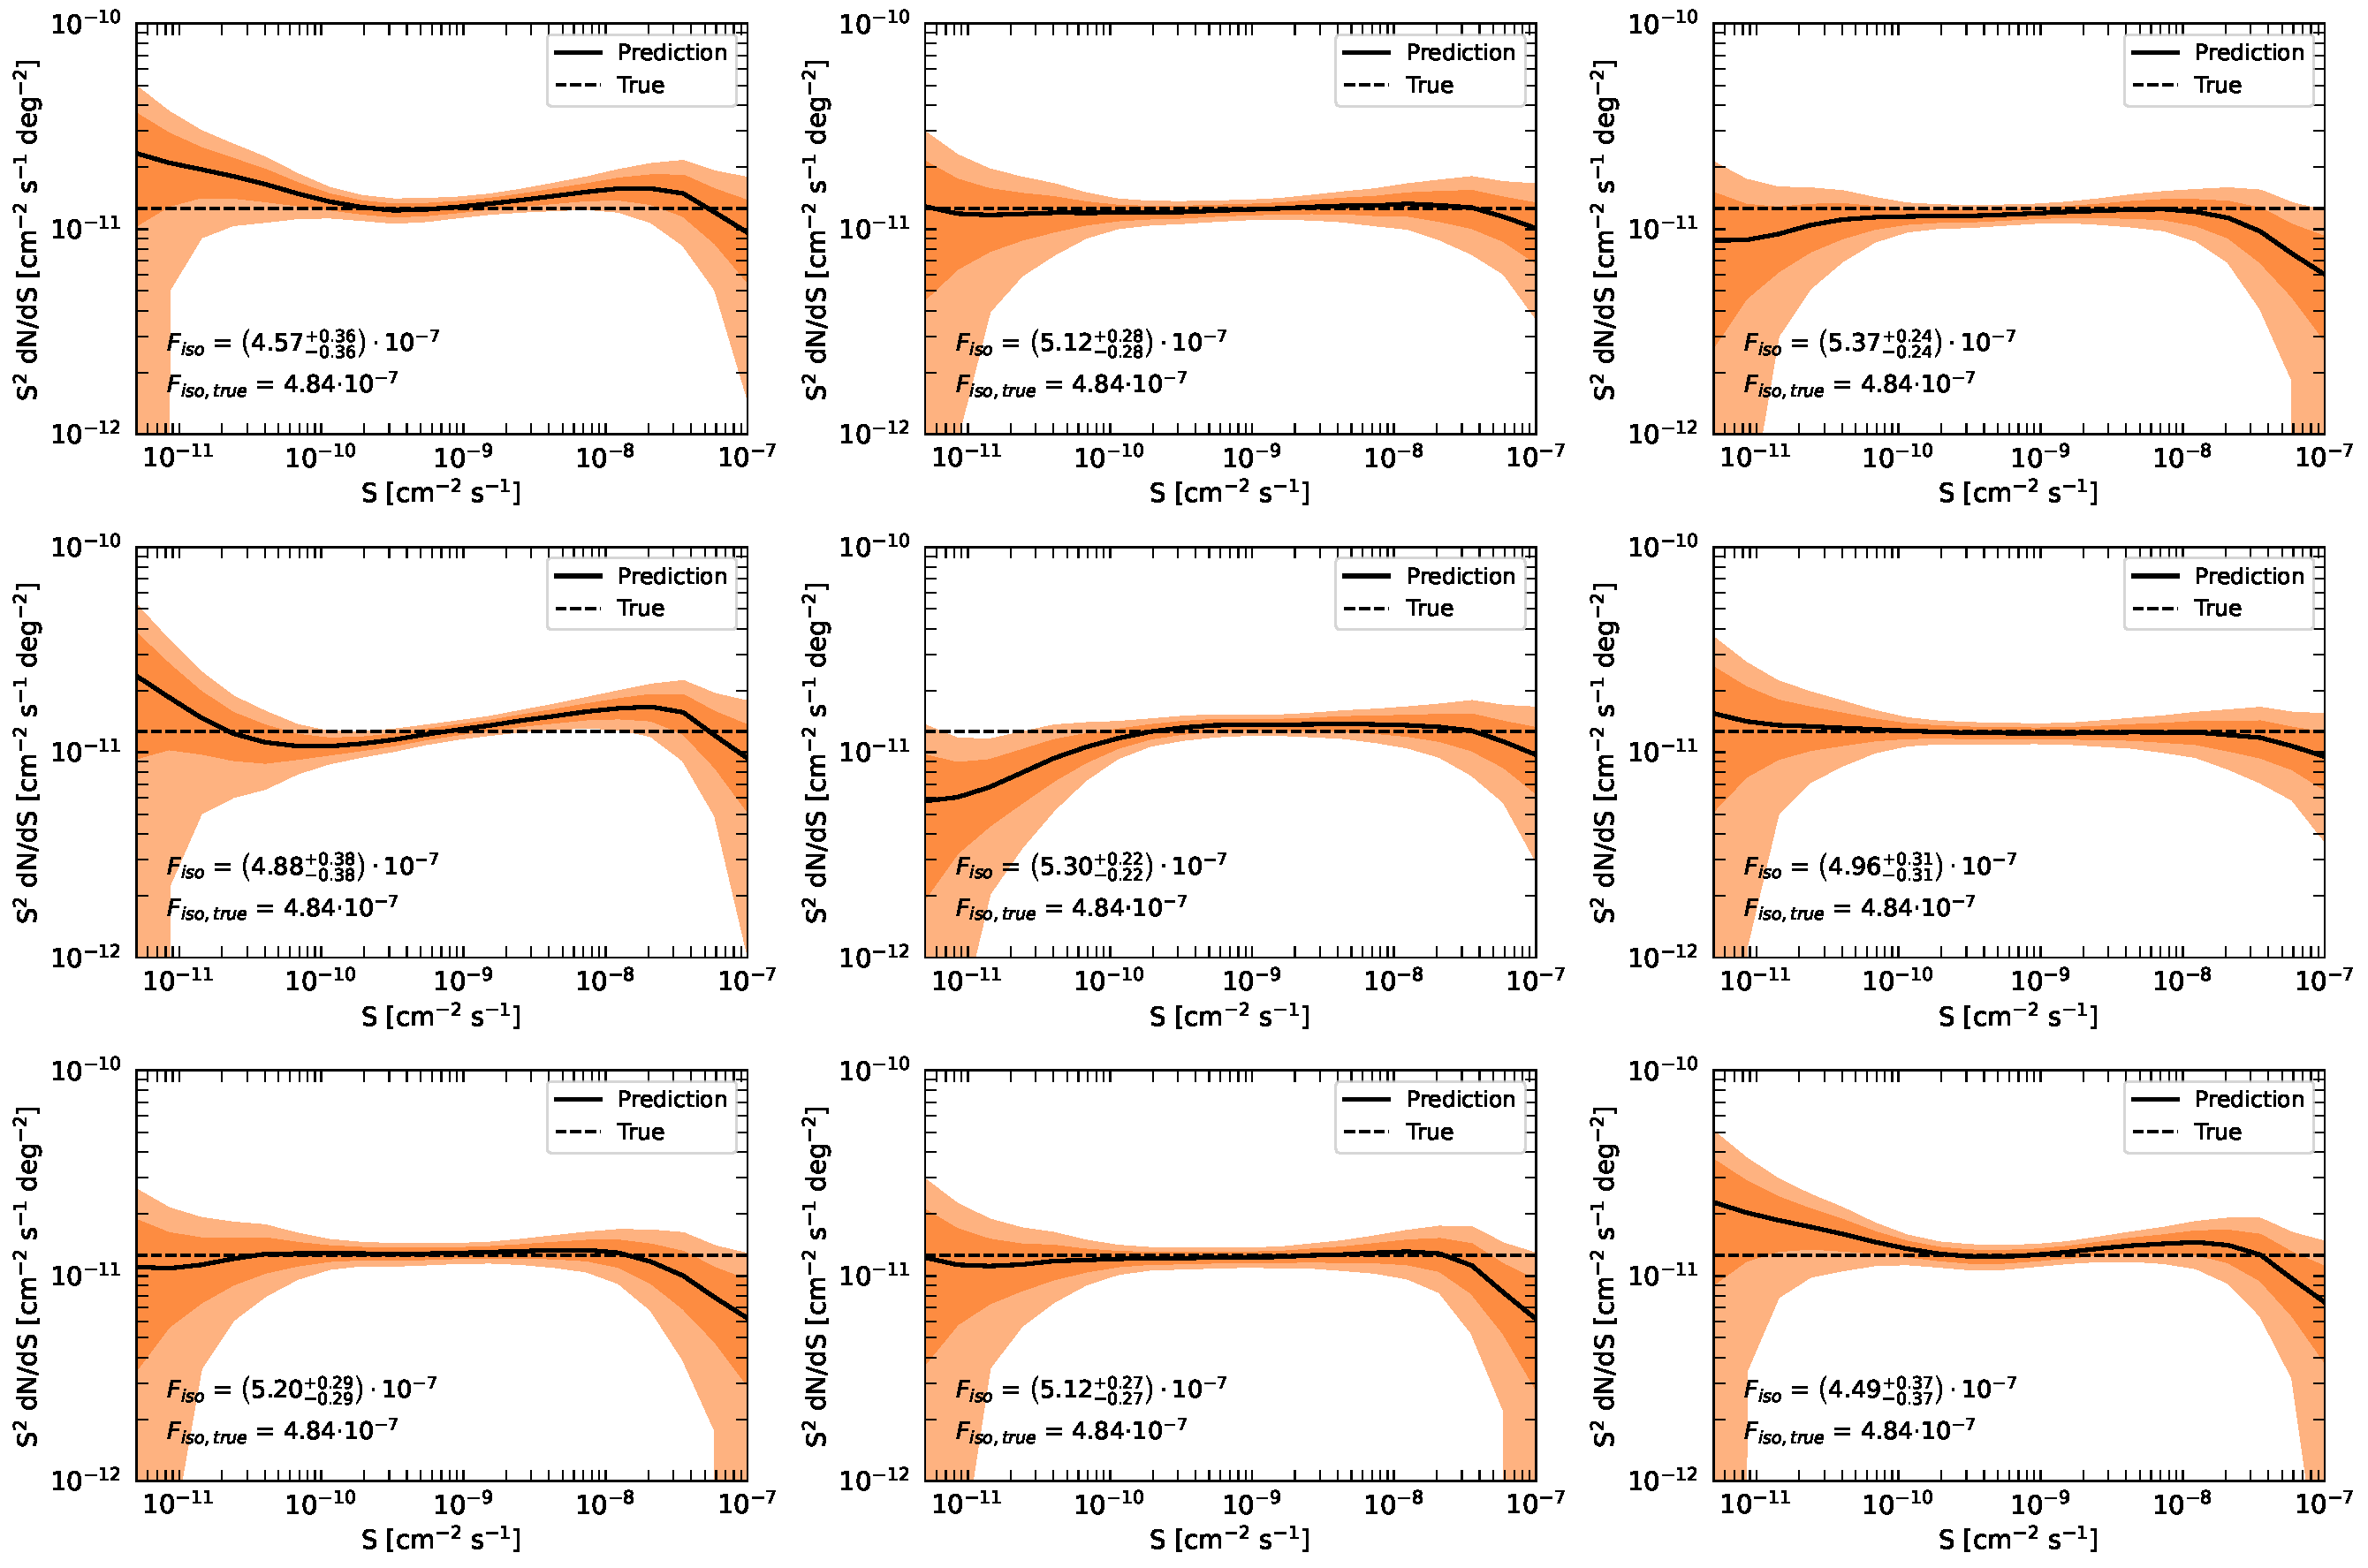
\includegraphics[width=1.0\textwidth]{chapter_06/sections/paper_dnds/img/model_plots/model_42/baseline/pendenza2.pdf}
\caption{  Same as Figure \ref{fig:random-maps}  but for 6 different random realization of the same flat $S^2\dnds$ and same $F_\textrm{iso,true}=4.84 \cdot 10^{-7}$ cm$^{-2}$ s$^{-1}$ sr$^{-1}$.  }
\label{fig:flat-maps}
\end{figure}

\begin{figure}[t]
\centering
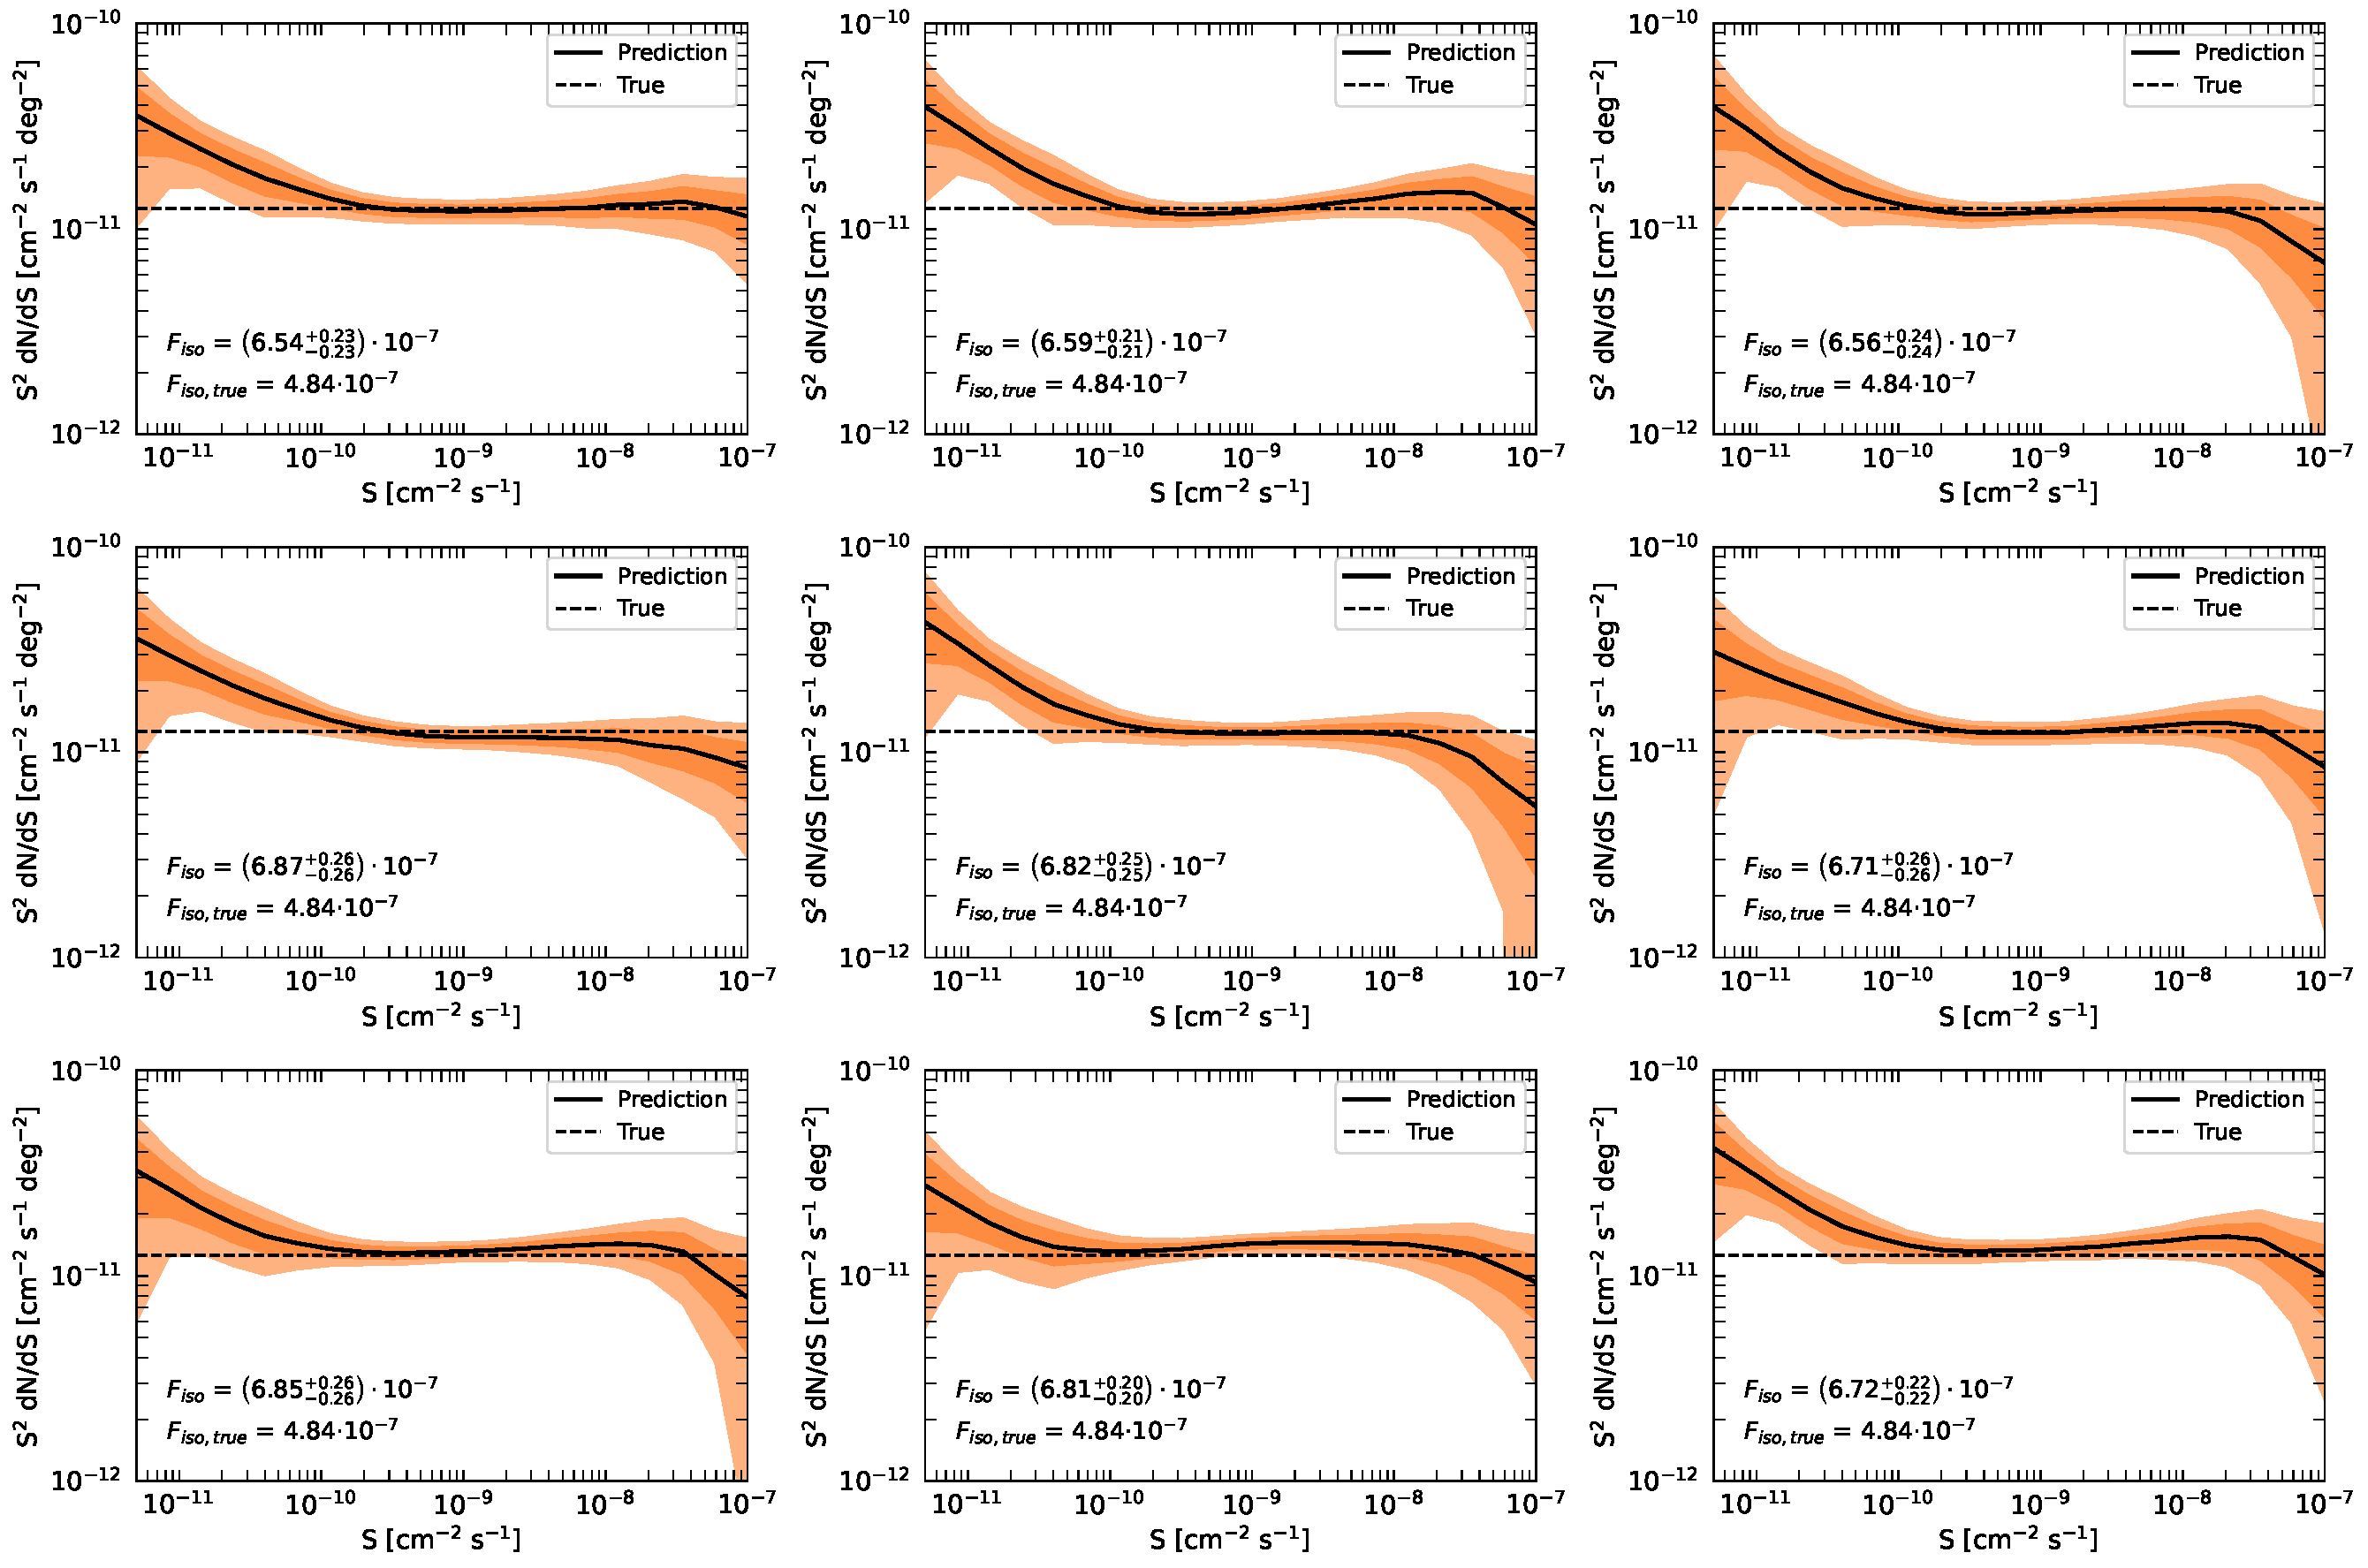
\includegraphics[width=1.0\textwidth]{chapter_06/sections/paper_dnds/img/model_plots/model_42/baseline/pendenza2-fg5.pdf}
\caption{
 Same as Figure \ref{fig:flat-maps} but for synthetic maps generated using version v05 of the foreground model.  }
\label{fig:flat-maps-v5}
\end{figure}


Figure \ref{fig:flat-maps} shows the stability of the CNN output for a specific repeated $\dnds$ input.
In this case, the CNN, trained on the wide variability of models of Table \ref{tab:prior-dNdS}, is applied to a set of maps, all generated with a specific $\dnds \sim S^{-2}$. This specific choice of input $\dnds$ is meant to test a case which is expected to be similar to the real \fermi case, as was found in \cite{Cuoco-1pdf} for mid-values of $S$. The plots show that the CNN is remarkably consistent in reproducing the correct behaviour. The drop at high fluxes is mostly due to the fact that the CNN has been instructed with maps that contain a dropping $\dnds$ at high fluxes (see Table \ref{tab:prior-dNdS} - the reason for this choice of prior is that sources in the 4FGL catalog exhibit this drop in the source count). For mid-values of $S$, the reconstructed $S^2\dnds$ is quite flat, with a small error band. At low $S$, well below the \fermi threshold and when approaching the confusion limit, some mild deviation occurs, but the true $\dnds$ lies always within the uncertainties. These tests gives us confidence that the CNN should be able to faithfully reconstruct the source distribution of the \fermi sky, when applied to the real data in Section \ref{sec:dnds:results}.

As a further test, we show in Figure \ref{fig:flat-maps-v5} the case where we apply our method to maps which contain a galactic foreground model different from the one used in the training. The CNN has been built (like in our baseline case) with maps generated with the galactic template model \verb|gll_iem_v07|. The same model is used in the foreground subtraction performed in the analysis. On the contrary, for this test we have generated maps  using the alternative \verb|gll_iem_v05| foreground model, and let the above \verb|gll_iem_v07|-trained CNN to analyze them. This has been done in order to verify the resilience of the method on the imperfect knowledge of the galactic foreground. Figure \ref{fig:flat-maps-v5} shows that the reconstructed $\dnds$ has a level of agreement with the input model comparable to the analogous case of Figure \ref{fig:flat-maps}. Some larger deviation is present at very low fluxes, even though the reconstructed and input models are compatible within $1\sigma$.




\subsubsection{UltraCleanVeto Selection} 


In this section we further test the robustness of the results to the \fermi data selection. In particular, while for the main results we used the \texttt{SOURCEVETO} event class selection, here we test the \texttt{ULTRACLEANVETO} selection. This event class has more stringent cuts with respct to the \texttt{SOURCEVETO} class, and it thus contains a lower residual charged  cosmic-ray background, at the prize of a lower effective area (by about 15\%). Except for the different data selection all the rest of the analysis is performed in the same identical way as for the \texttt{SOURCEVETO} case. The resulting $\dnds$ is shown in Figure \ref{fig:prediction-fermi-12y-ucv} and it can be seen that it is compatible with the main results, while, as expected, the value of $\fiso$ is a bit lower. 



\subsubsection{Multipole Analysis}



Since foreground modeling can be an important source of systematic uncertainty,  we investigate this potential issue performing a further test. 
As discussed above, the signal we try to extract from the gamma ray maps, is a small-scale effect, since it is due to a distribution of point sources. To a large degree, this point sources are isotropically distributed in the sky and contribute to the fluctuations of this isotropic field at small angular scales. On the contrary, the galactic foreground is quite diffuse, as can be seen in Figure \ref{fig:galactic-foreground}, and therefore contributes mainly to large-scale anisotropies. 
In order to further remove from the data the possible large-scale residual component of the galactic foreground, which might still be present after imperfect foreground removal performed with the use of the templates, we adopt a method based on the transformation of the flux to harmonic space and the removal from the maps of the low-multipoles (i.e., large angular scales) contribution. 
We stress that this procedure is applied only to the \fermi data map, and  not to the synthetic maps. For the latter, the foreground subtracted is the same used to generate the maps, so foreground subtraction is, by definition, ``perfect''. 
The procedure follows these steps:

\begin{itemize}
\item We start with the foreground-subtracted flux map, to which we apply the $|b|<30^\circ$ latitude cut and a $2^\circ$ mask around each of the bright sources of the 4FGL catalog (which would otherwise dominate the angular power spectrum).
We first determine and remove the monopole ($l=0$) and dipole ($l=1$) components from the masked map (for this, we use the \verb|remove_dipole| routine from the Healpy library). In this way, after the subtraction procedure outlined below, the monopole (i.e. the total flux) and dipole information of the \fermi map are retained.

\item  This map is then subject to harmonic space decomposition:
\begin{equation}
\mathcal{M}_\textrm{masked}(\theta,\phi) = \sum_{l=0}^{\infty} \sum_{m=-l}^{l} a_{lm} Y_{lm}(\theta,\phi)
\label{eq:multipole}
\end{equation}
where $\theta$ and $\phi$ are angles on the sphere, $Y_{lm}(\theta,\phi)$ the spherical harmonics and the harmonic coefficients $a_{lm}$ completely encode the same information present in the map $\mathcal{M}_\textrm{masked}$  (notice that, even though in Eq. (\ref{eq:multipole}) we formally decompose over all multipoles, the monopole and dipole amplitude are vanishing, since they have been removed from  $\mathcal{M}_\textrm{masked}$);

\item The harmonic coefficients $a_{lm}$ are determined with the \verb|map2alm| Healpy function. The ones that are retained for the foreground cleaning are those referring to multipole values $l < l_\textrm{max}$, where $l_\textrm{max}$ will be varied and the dependence of the results with $l_\textrm{max}$ will be studied (at this level, the monopole and dipole are not present, because of the above point);

\item By using the $a_{lm}$ corresponding to multipoles $l < l_\textrm{max}$, we use Eq. (\ref{eq:multipole}) to construct a map $\mathcal{M}_\textrm{residual}$ which contains only the large-scale component. This is performed with \verb|alm2map| Healpy function.

\item We subtract the residual map from the original map, thus obtaining a map where the large scale residual components have been removed. The size of the scale is determined by $l < l_\textrm{max}$.

\end{itemize}

With this algorithm we obtain maps where the large scale residual features associated to imperfect  galactic foreground subtraction are further removed. The results we obtain on the reconstructed $\dnds$ for the \fermi data (after this ``multipole cleaning") are shown in Figure \ref{fig:multipole-cleaningv7}, for different values of $l_\textrm{max}$ and for the \verb|gll_iem_v07| template. By comparing Figure \ref{fig:multipole-cleaningv7} with Figure \ref{fig:prediction-fermi-12y}, which refers to the same foreground template and latitude cut, we can see that the results are extremely stable up to $l_\textrm{max} \sim 100$. This means that our baseline analysis is not affected by incomplete foreground subtraction, and can be considered reliable.
The fall-off of the $\dnds$ when $l_\textrm{max} > 100$ is expected 
since $l_\textrm{max} = 100$
corresponds to an angular scale of the order of $2^\circ$, 
which starts to be compatible with the size of (PSF-smeared) point sources. Therefore, a cleaning with $l_\textrm{max} > 100$ starts to remove point sources instead of galactic foregrounds.

The same analysis has been performed on a pipeline fully based on  \verb|gll_iem_v05|: the result is shown in Figure \ref{fig:multipole-cleaningv5}, to be compared with Figure \ref{fig:prediction-fermi-12y-fg-v5}. Also in this case, the results are extremely stable up to $l_\textrm{max} \sim 100$, and the same above considerations apply.

Finally, to check the strength of the method against the imperfect knowledge of the background, we performed the same analysis of multipole cleaning by adopting our baseline pipeline (based on \verb|gll_iem_v07|) on maps generated with \verb|gll_iem_v05| (similarly to what has been done for  Figure \ref{fig:flat-maps-v5}). The results are shown in Figure \ref{fig:multipole-cleaning-v5-and-v7} , where again we see that the results are pretty consistent, up to $l\sim 100$.
 It can be seen, moreover, that the procedure of multipole cleaning helps in removing the, nonetheless small, positive bias which is present toward low fluxes in this case.  

In conclusion, these tests give confidence on the reliability of the method and that the main result of Figure \ref{fig:prediction-fermi-12y} corresponds to a fair representation of the source-count distribution of the unresolved gamma-ray sources.



\begin{figure}[t]
\centering
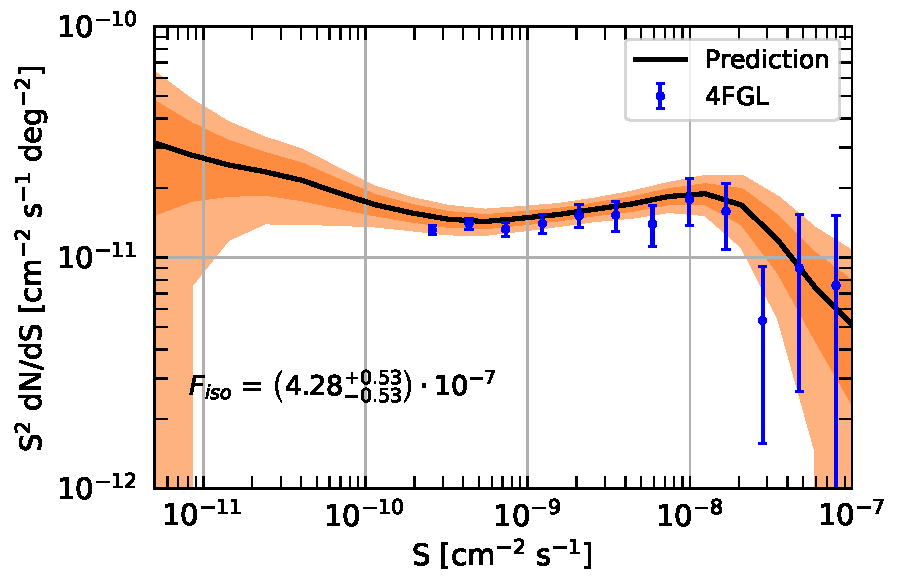
\includegraphics[width=0.9\textwidth]{chapter_06/sections/paper_dnds/img/model_plots/model_42/UCV/fermi_prediction_hs.pdf}
\caption{Same as Figure \ref{fig:prediction-fermi-12y} but  for the \texttt{ULTRACLEANVETO}  \fermi data selection. }
\label{fig:prediction-fermi-12y-ucv}
\end{figure}






\begin{figure}[t]
\centering
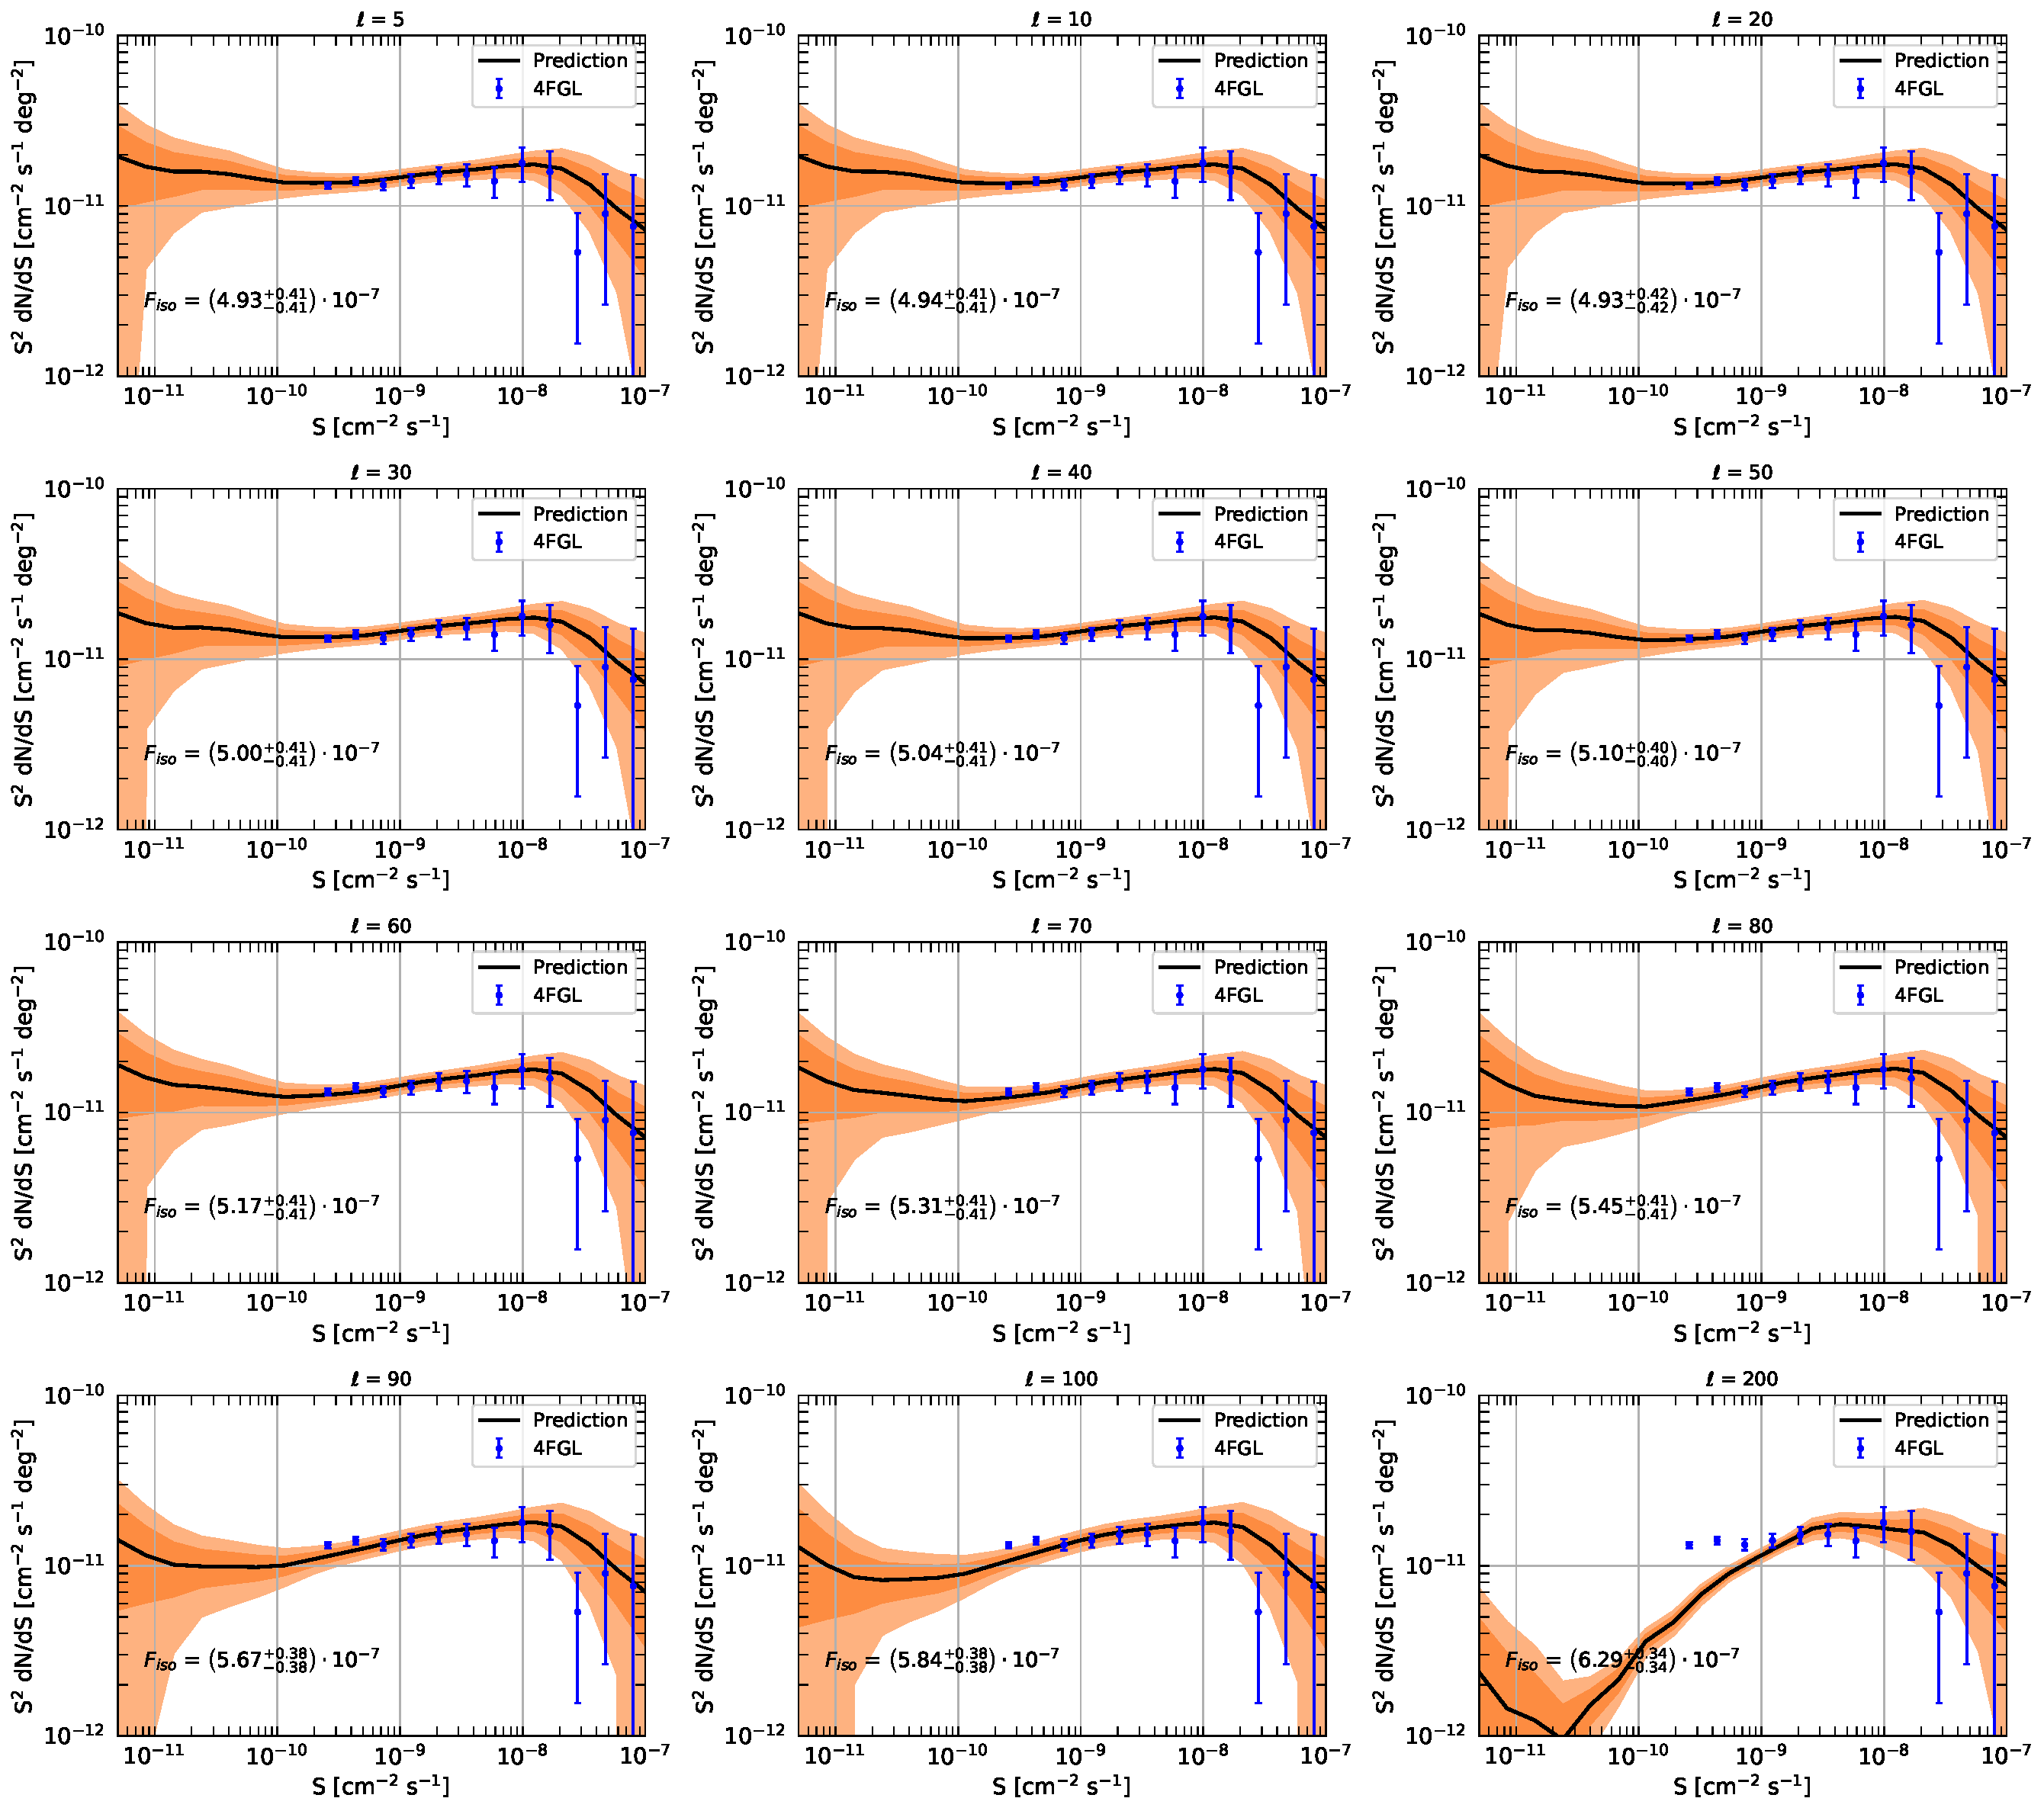
\includegraphics[width=1.0\textwidth]{chapter_06/sections/paper_dnds/img/model_plots/model_42/baseline/fermi_map_cleaning.pdf}
\caption{Same as Figure \ref{fig:prediction-fermi-12y} but where the \fermi map given as input to the CNN has been processed with the improved foreground cleaning procedure based on multipole decomposition described in the text. Each panel refer to a different maximal multipole $\ell_{max}$ used for the cleaning.  }
\label{fig:multipole-cleaningv7}
\end{figure}

\begin{figure}[t]
\centering
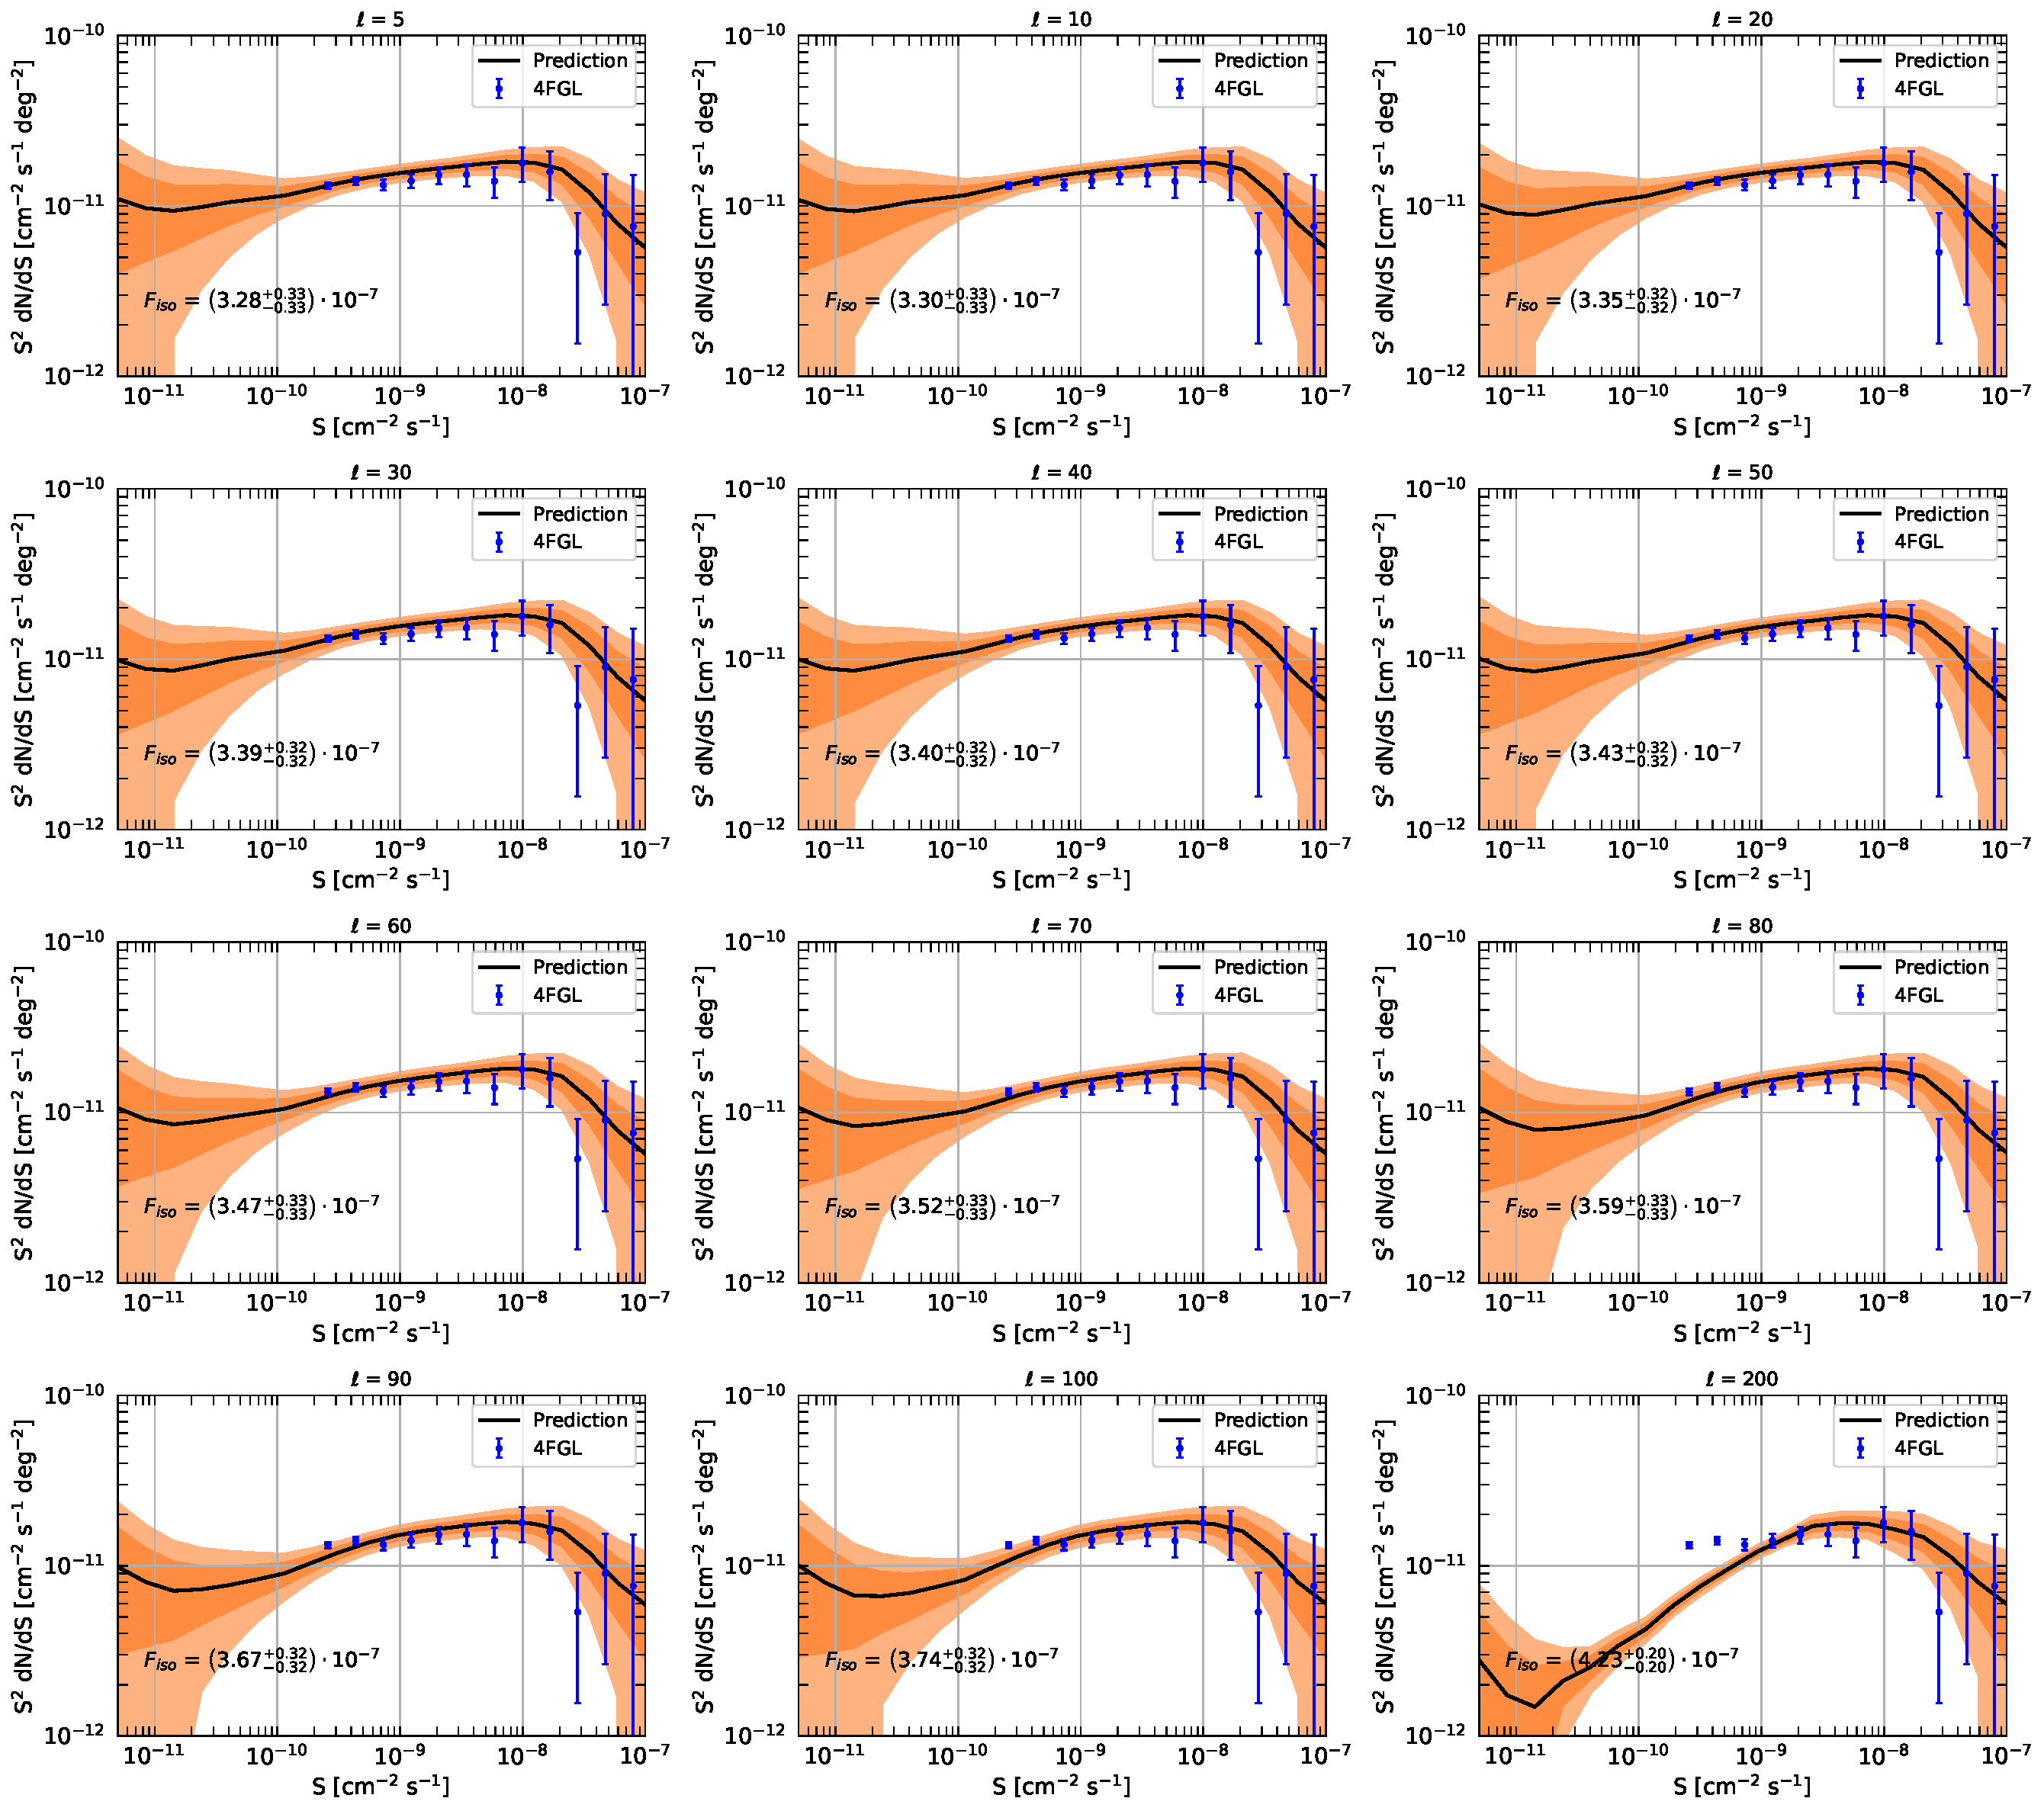
\includegraphics[width=1.0\textwidth]{chapter_06/sections/paper_dnds/img/model_plots/model_42/fg5/fermi_map_cleaning.pdf}
\caption{Same as Figure \ref{fig:multipole-cleaningv7} but using a CNN trained with the v05 version of the foreground model, as well as using as input a \fermi count map processed with the same foreground model.}
\label{fig:multipole-cleaningv5}
\end{figure}

\begin{figure}[t]
\centering
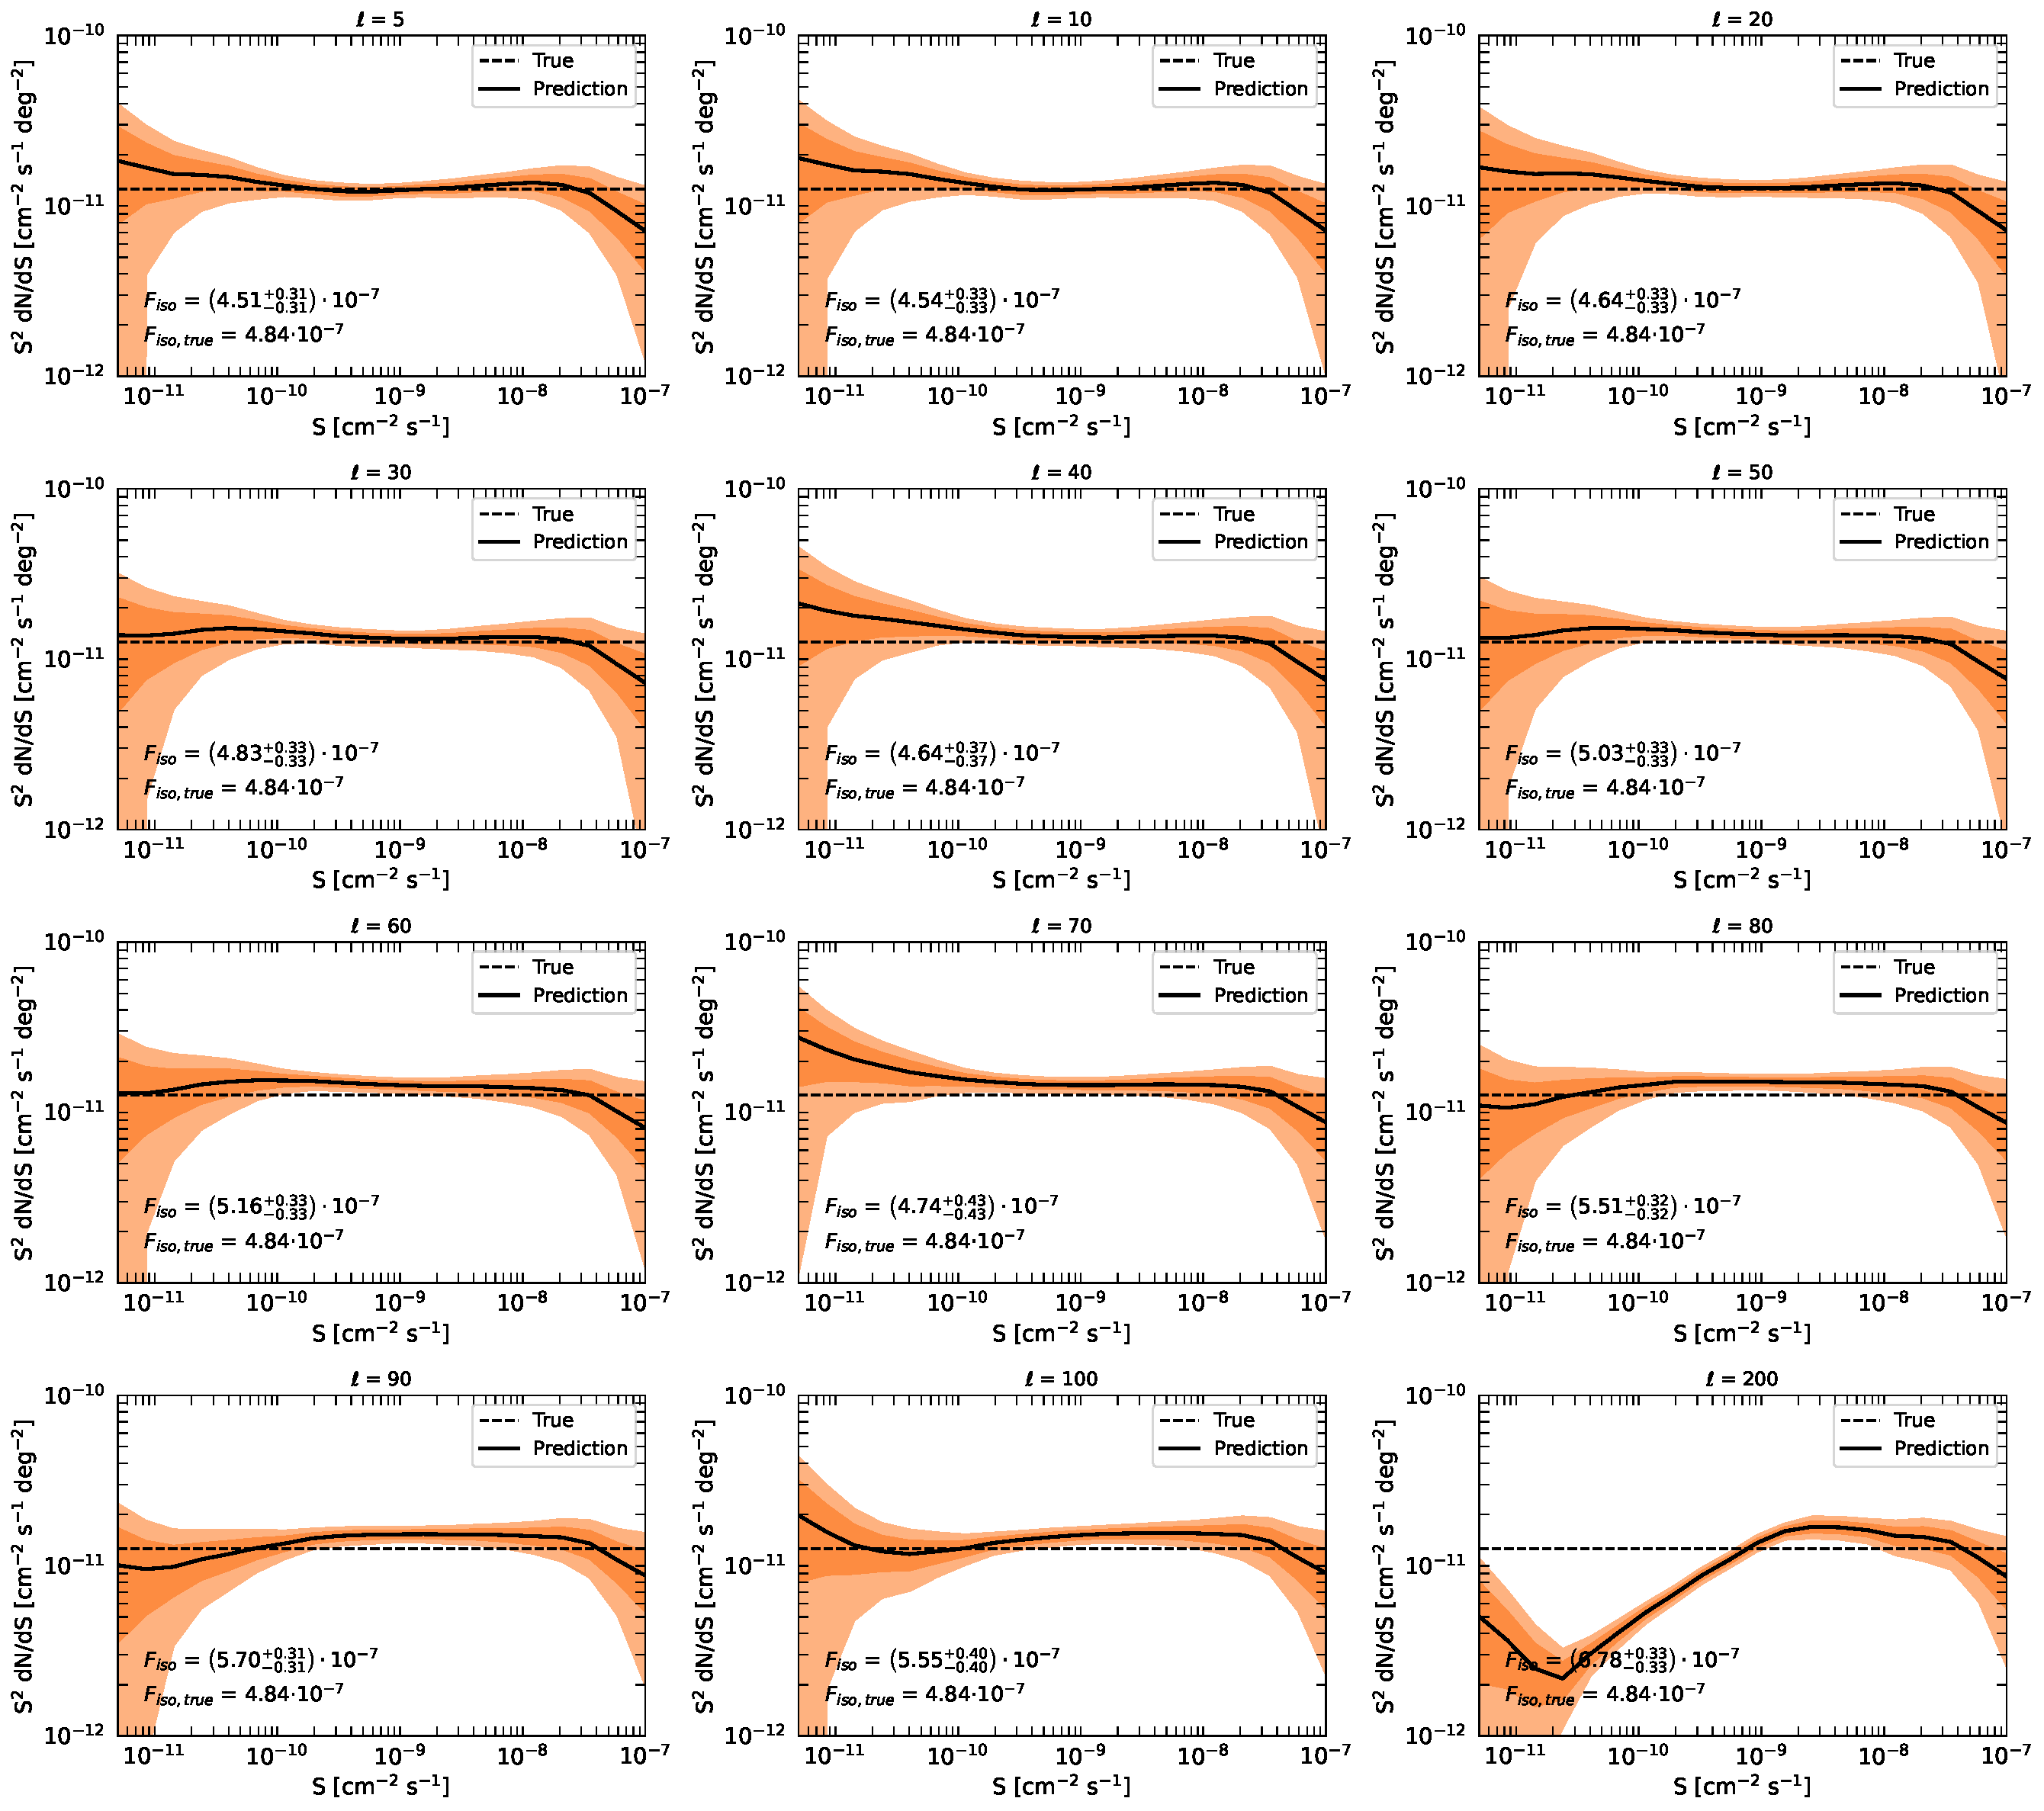
\includegraphics[width=1.0\textwidth]{chapter_06/sections/paper_dnds/img/model_plots/model_42/baseline/syn_flat_map_fg5.pdf}
\caption{Same as Figure \ref{fig:multipole-cleaningv7} but using as input a synthetic map generated with a flat $S^2 \dnds$ and with the v05 version of the foreground model.}
\label{fig:multipole-cleaning-v5-and-v7}
\end{figure}



\subsubsection{Changing $A_\textrm{gal}$}
\label{sec:agal-var}

In order to test the stability of the results against changes in the values of $A_\textrm{gal}$, we have provided, as input to our trained CNN, \fermi maps cleaned with different values of $A_\textrm{gal}$, ranging from 0.78 to 1.0 (our fiducial value is $0.888 \pm 0.005$, thus the chosen range encompass many standard deviations around its central value). The results are shown in Figure \ref{fig:Agal_change} below. It can be seen that the $dN/dS$ is considerably robust and stable to different values of $A_\textrm{gal}$, despite the large range explored. Instead, different values of $A_\textrm{gal}$ seem to imply a significant variation in the reconstructed value of $F_\textrm{iso}$, as expected since at the large Galactic latitudes explored in our analysis ($|b| > 30^\circ$) there is a certain amount of degeneracy between a purely isotropic emission and the Galactic foreground emission itself. However, this does not affect the reconstructed $dN/dS$.



\subsubsection{Fully spherical CNN}
\label{sec:full-spherical-nn}

In this section we show a comparison of the results obtained using a fully spherical CNN, instead of the \verb|map2patch| algorithm used in the main analysis. In particular, we adopt here the NNHealpix \cite{Krachmalnicoff:2019} algorithm.

Figure \ref{fig:SphericalNN-Fermi-dnds} shows the reconstructed $\dnds$, $\fiso$  and their frequentist errors, using the spherical CNN applied to the \fermi map. The results are fully compatible with the ones obtained with the \verb|map2patch| algorithm, both for the mean value and the errors, as can be seen by confronting with Figure \ref{fig:prediction-fermi-12y-bayesian}.


Figure \ref{fig:SphericalNN-test-random} instead, shows some examples of random input $\dnds$ and $\fiso$ from the validation dataset of the Spherical CNN, and the corresponding quantities and their errors reconstructed by the CNN.
The spherical CNN has similar performances as the  CNN that uses \verb|map2patch|, as can be seen comparing with Figure \ref{fig:random-maps}. The same occurs also in Figure \ref{fig:SphericalNN-test-flat}, which refers to a flat $S^2 dN/dS$, to be compared with Figure \ref{fig:flat-maps} obtained with \verb|map2patch|.

%{\blue AA: non dovrebbe essere un confronto tra fig \ref{fig:SphericalNN-test-flat} e fig \ref{fig:flat-maps}?}





\begin{figure}[t]
\centering
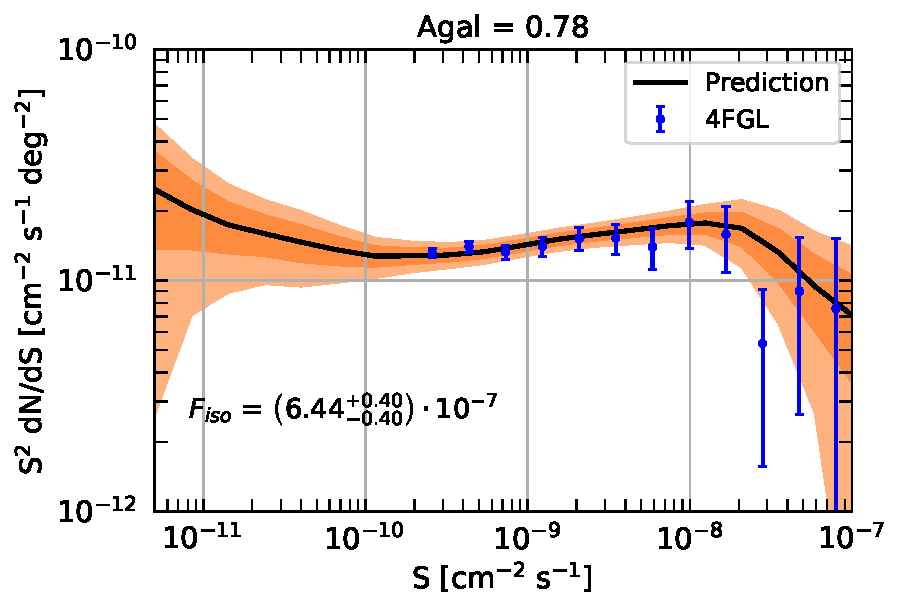
\includegraphics[width=0.45\textwidth]{chapter_06/sections/paper_dnds/img/model_plots/model_42/baseline/Agal/fermi_prediction_Agal_0.780000.pdf}
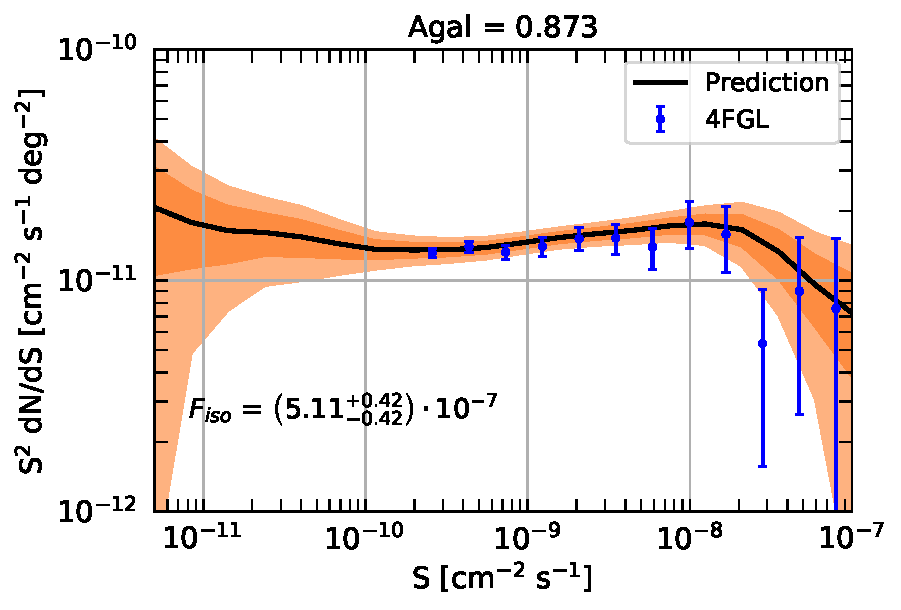
\includegraphics[width=0.45\textwidth]{chapter_06/sections/paper_dnds/img/model_plots/model_42/baseline/Agal/fermi_prediction_Agal_0.873000.pdf}
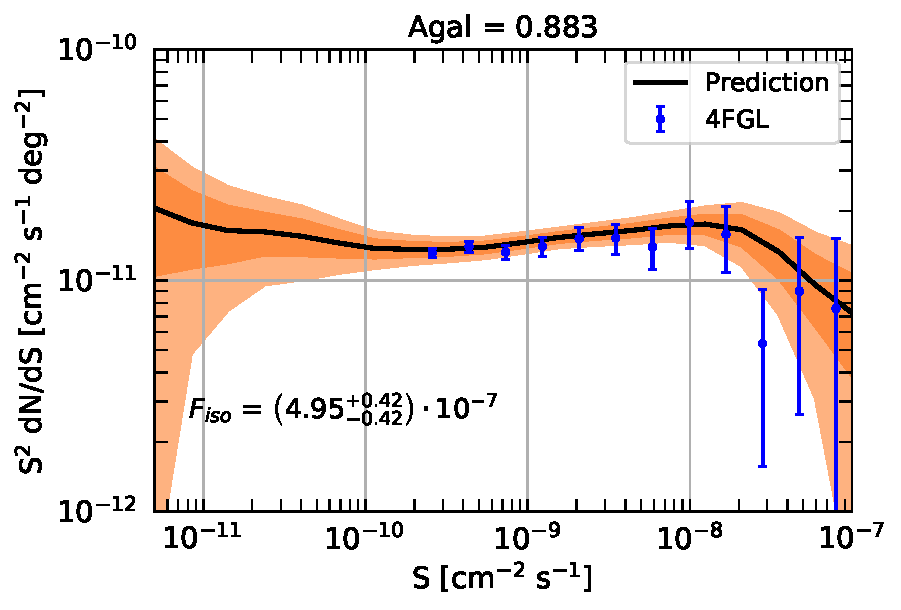
\includegraphics[width=0.45\textwidth]{chapter_06/sections/paper_dnds/img/model_plots/model_42/baseline/Agal/fermi_prediction_Agal_0.883000.pdf}
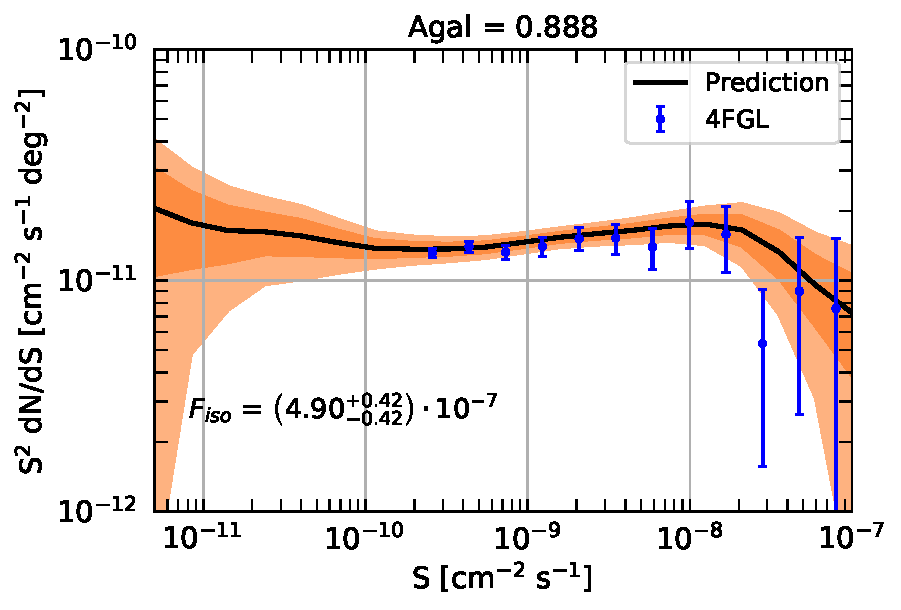
\includegraphics[width=0.45\textwidth]{chapter_06/sections/paper_dnds/img/model_plots/model_42/baseline/Agal/fermi_prediction_Agal_0.888000.pdf}
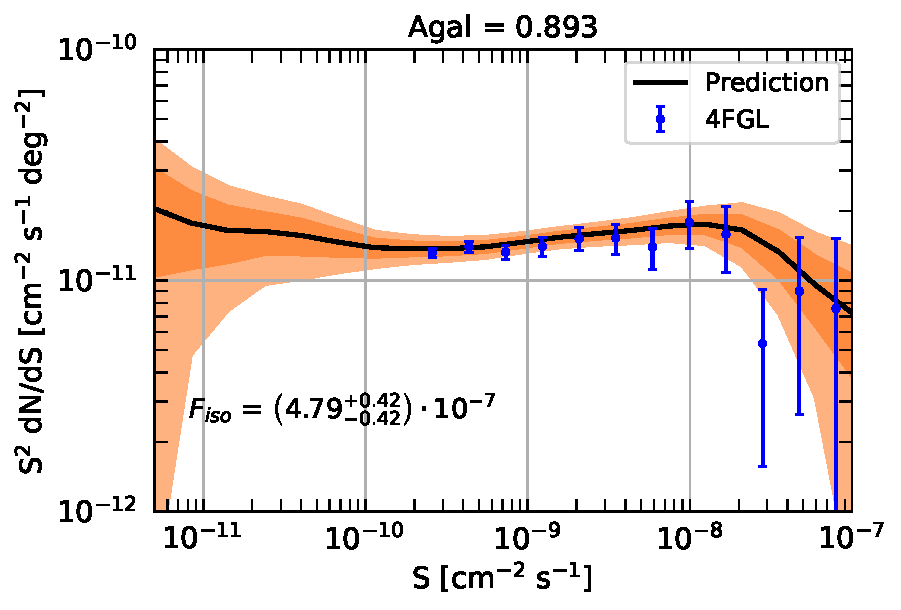
\includegraphics[width=0.45\textwidth]{chapter_06/sections/paper_dnds/img/model_plots/model_42/baseline/Agal/fermi_prediction_Agal_0.893000.pdf}
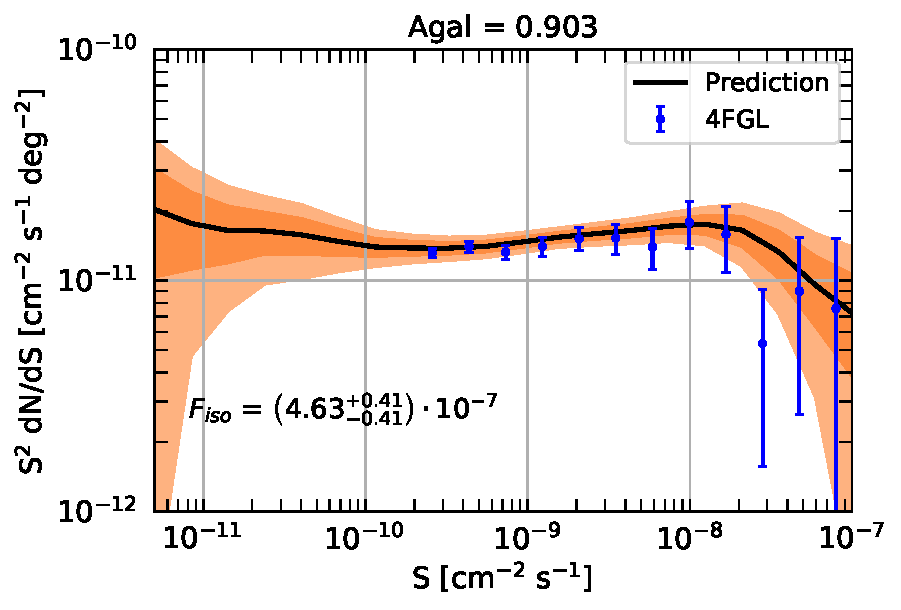
\includegraphics[width=0.45\textwidth]{chapter_06/sections/paper_dnds/img/model_plots/model_42/baseline/Agal/fermi_prediction_Agal_0.903000.pdf}
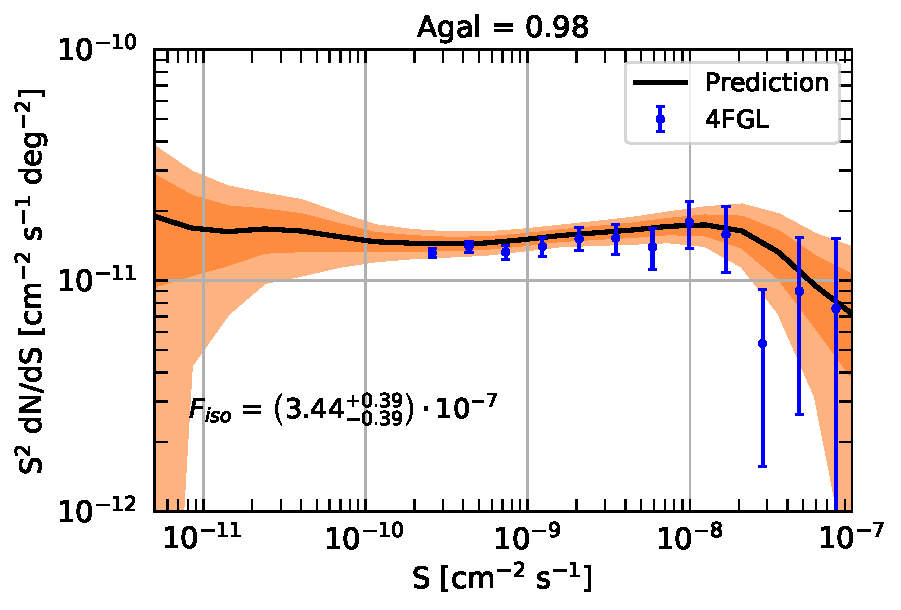
\includegraphics[width=0.45\textwidth]{chapter_06/sections/paper_dnds/img/model_plots/model_42/baseline/Agal/fermi_prediction_Agal_0.980000.pdf}
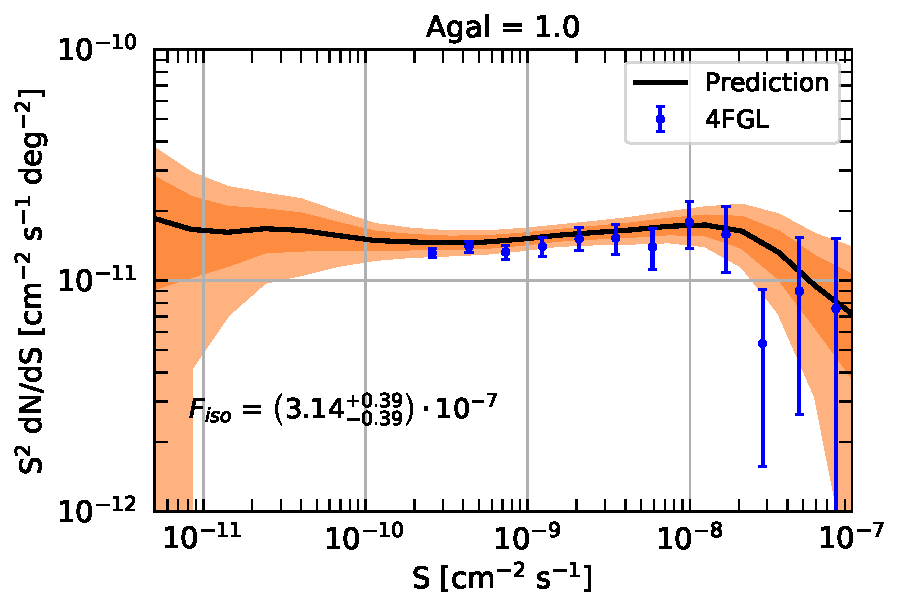
\includegraphics[width=0.45\textwidth]{chapter_06/sections/paper_dnds/img/model_plots/model_42/baseline/Agal/fermi_prediction_Agal_1.000000.pdf}
\caption{%Same as Figure \ref{fig:prediction-fermi-12y} 
Reconstructed $\dnds$ and $\fiso$  and their Bayesian errors, when the trained CNN is applied to the \fermi map  using  different values of $A_\textrm{gal}$ as indicated in the panel labels.}
\label{fig:Agal_change}
\end{figure}





\begin{figure}[t]
\centering
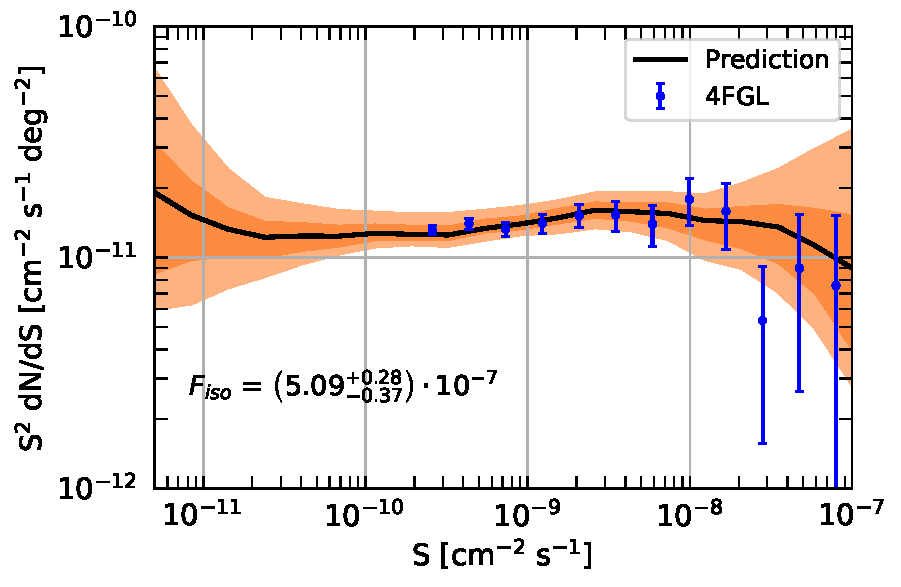
\includegraphics[width=0.9\textwidth]{chapter_06/sections/paper_dnds/img/model_plots/model_42/spherical/fermi_prediction_hist.pdf}
\caption{Reconstructed $\dnds$ and $\fiso$  and their errors, using a fully spherical  CNN, trained on simulated maps and then applied to the \fermi map. }
\label{fig:SphericalNN-Fermi-dnds}
\end{figure}



\begin{figure}[t]
\centering
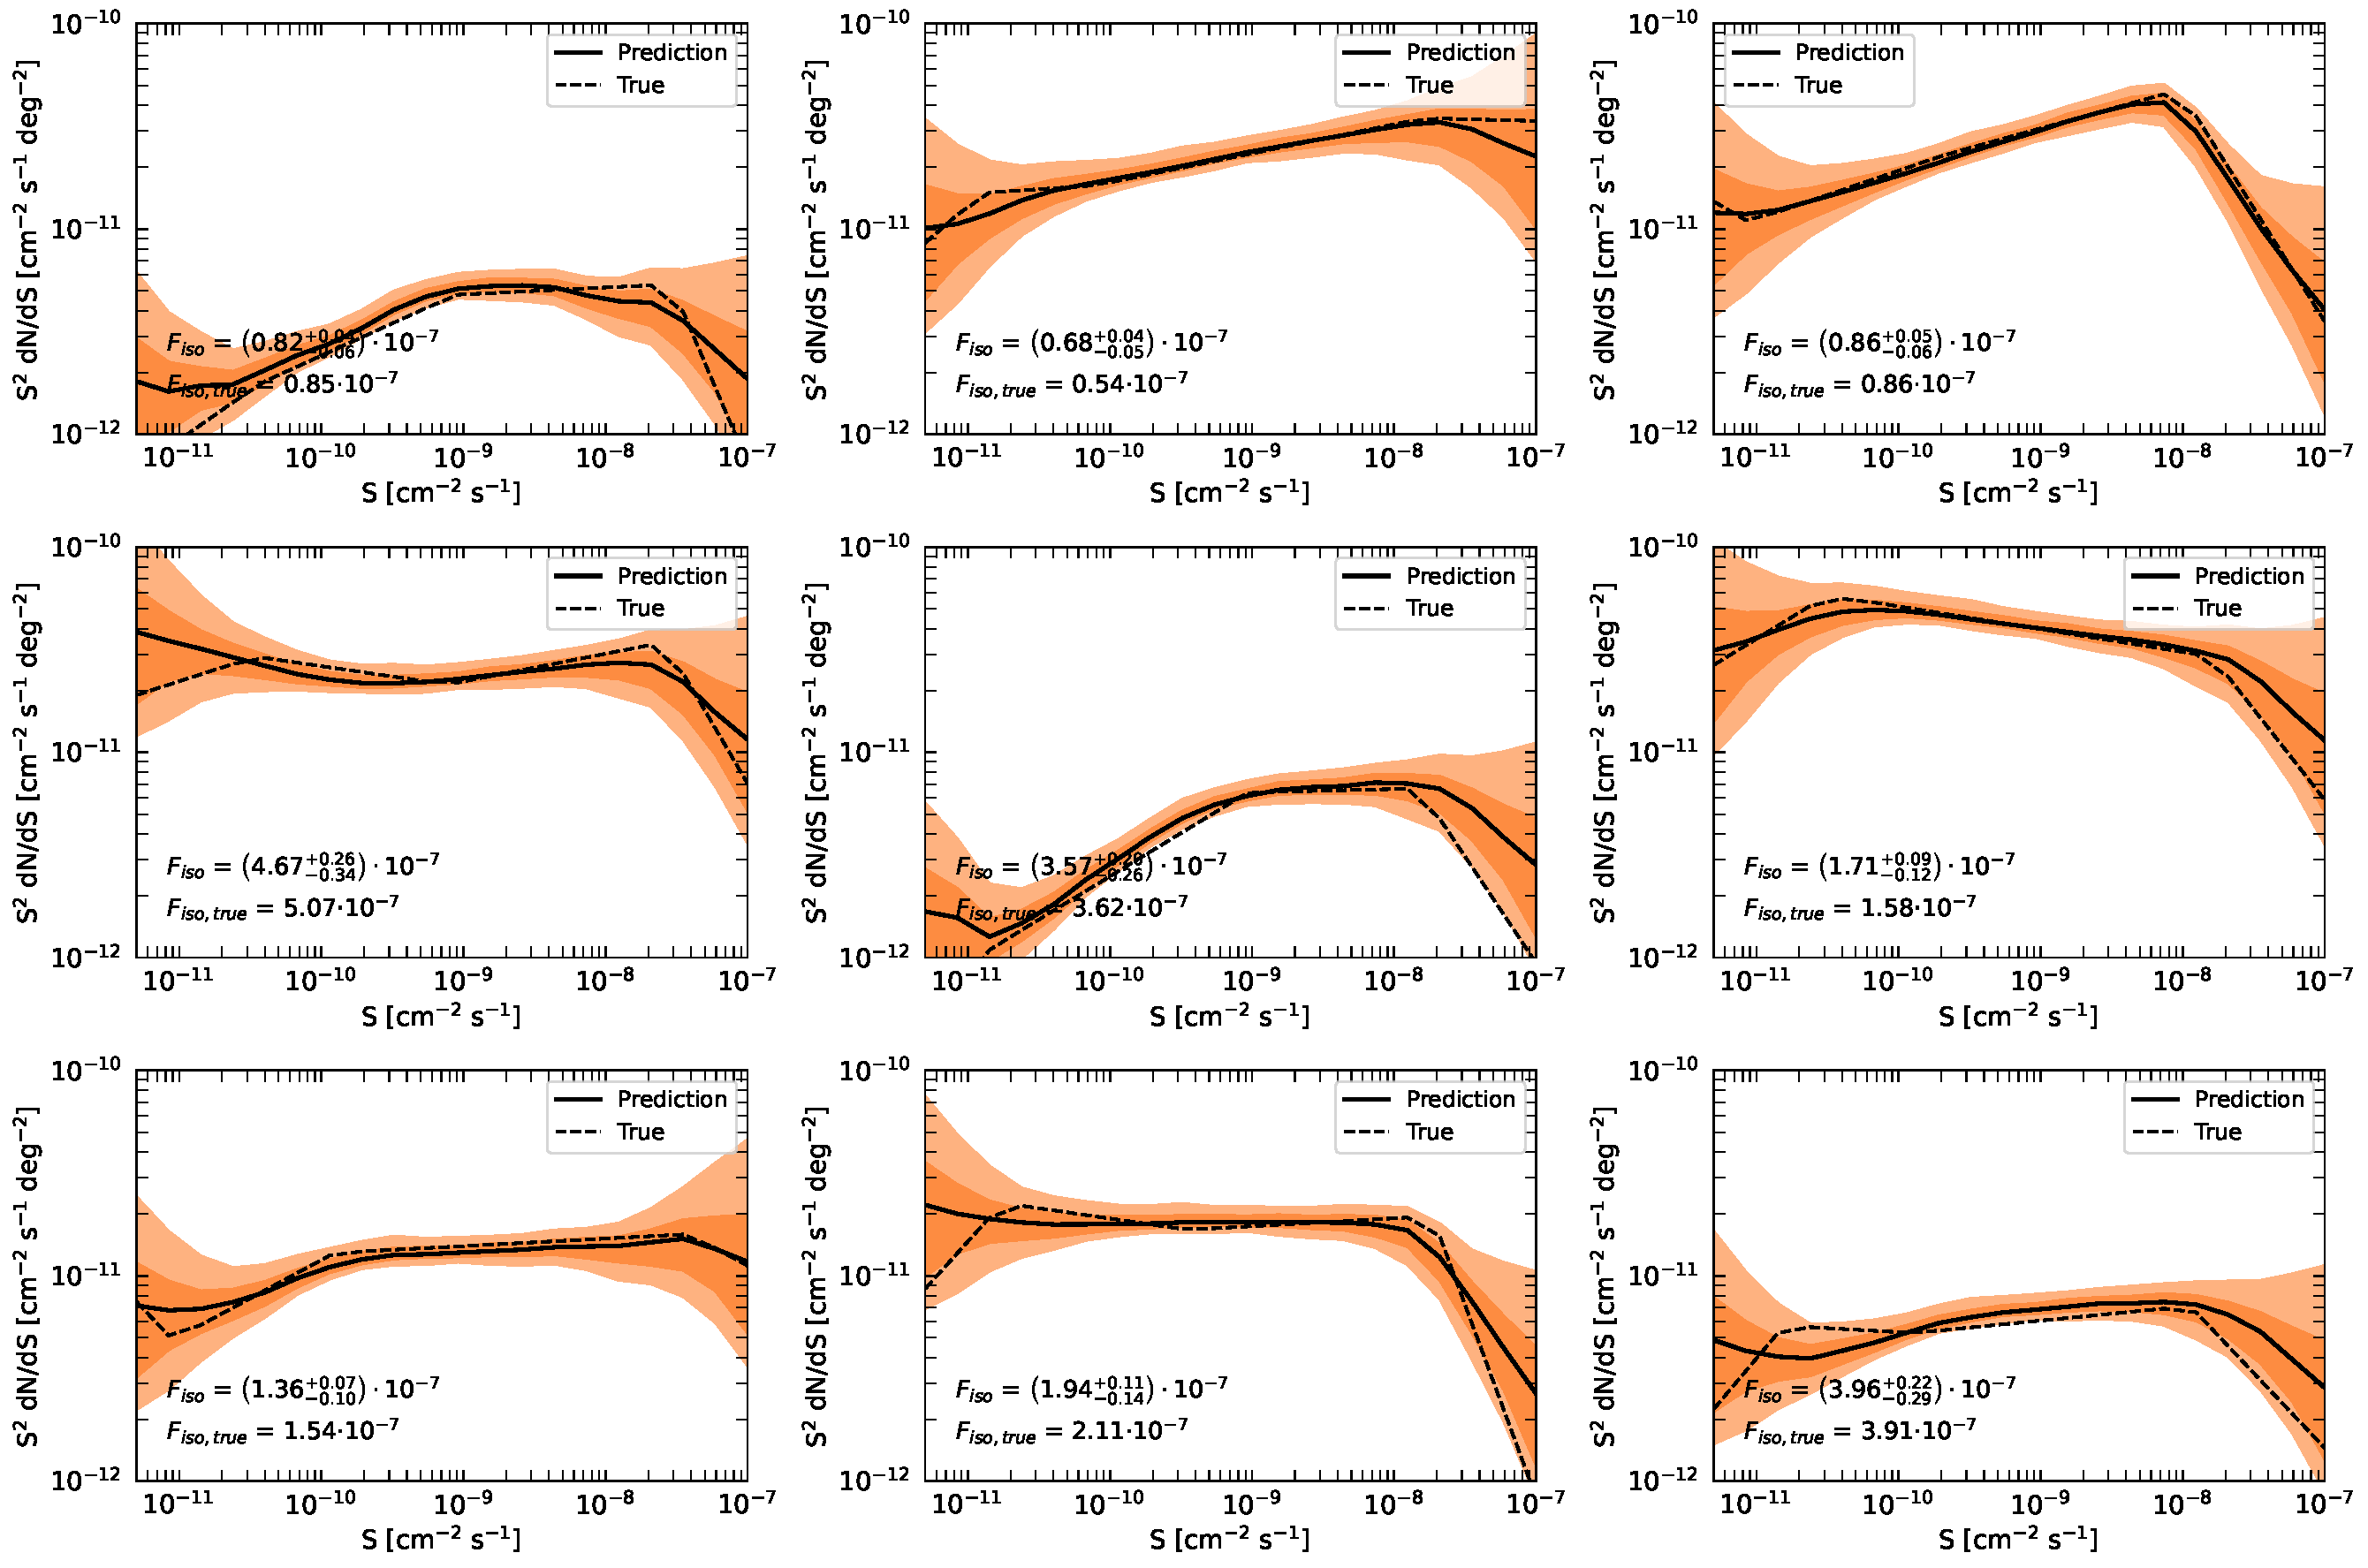
\includegraphics[width=1.0\textwidth]{chapter_06/sections/paper_dnds/img/model_plots/model_42/spherical/model_42_7i2_n64_sp_HL_predictions.pdf}
\caption{Some example $\dnds$ from the validation dataset of the spherical CNN. Each panel shows the input $\dnds$ and $\fiso$ and the corresponding quantities reconstructed by the CNN. The colored areas indicate the $1\sigma$ and $2\sigma$ uncertainty bands. }
\label{fig:SphericalNN-test-random}
\end{figure}





\begin{figure}[t]
\centering
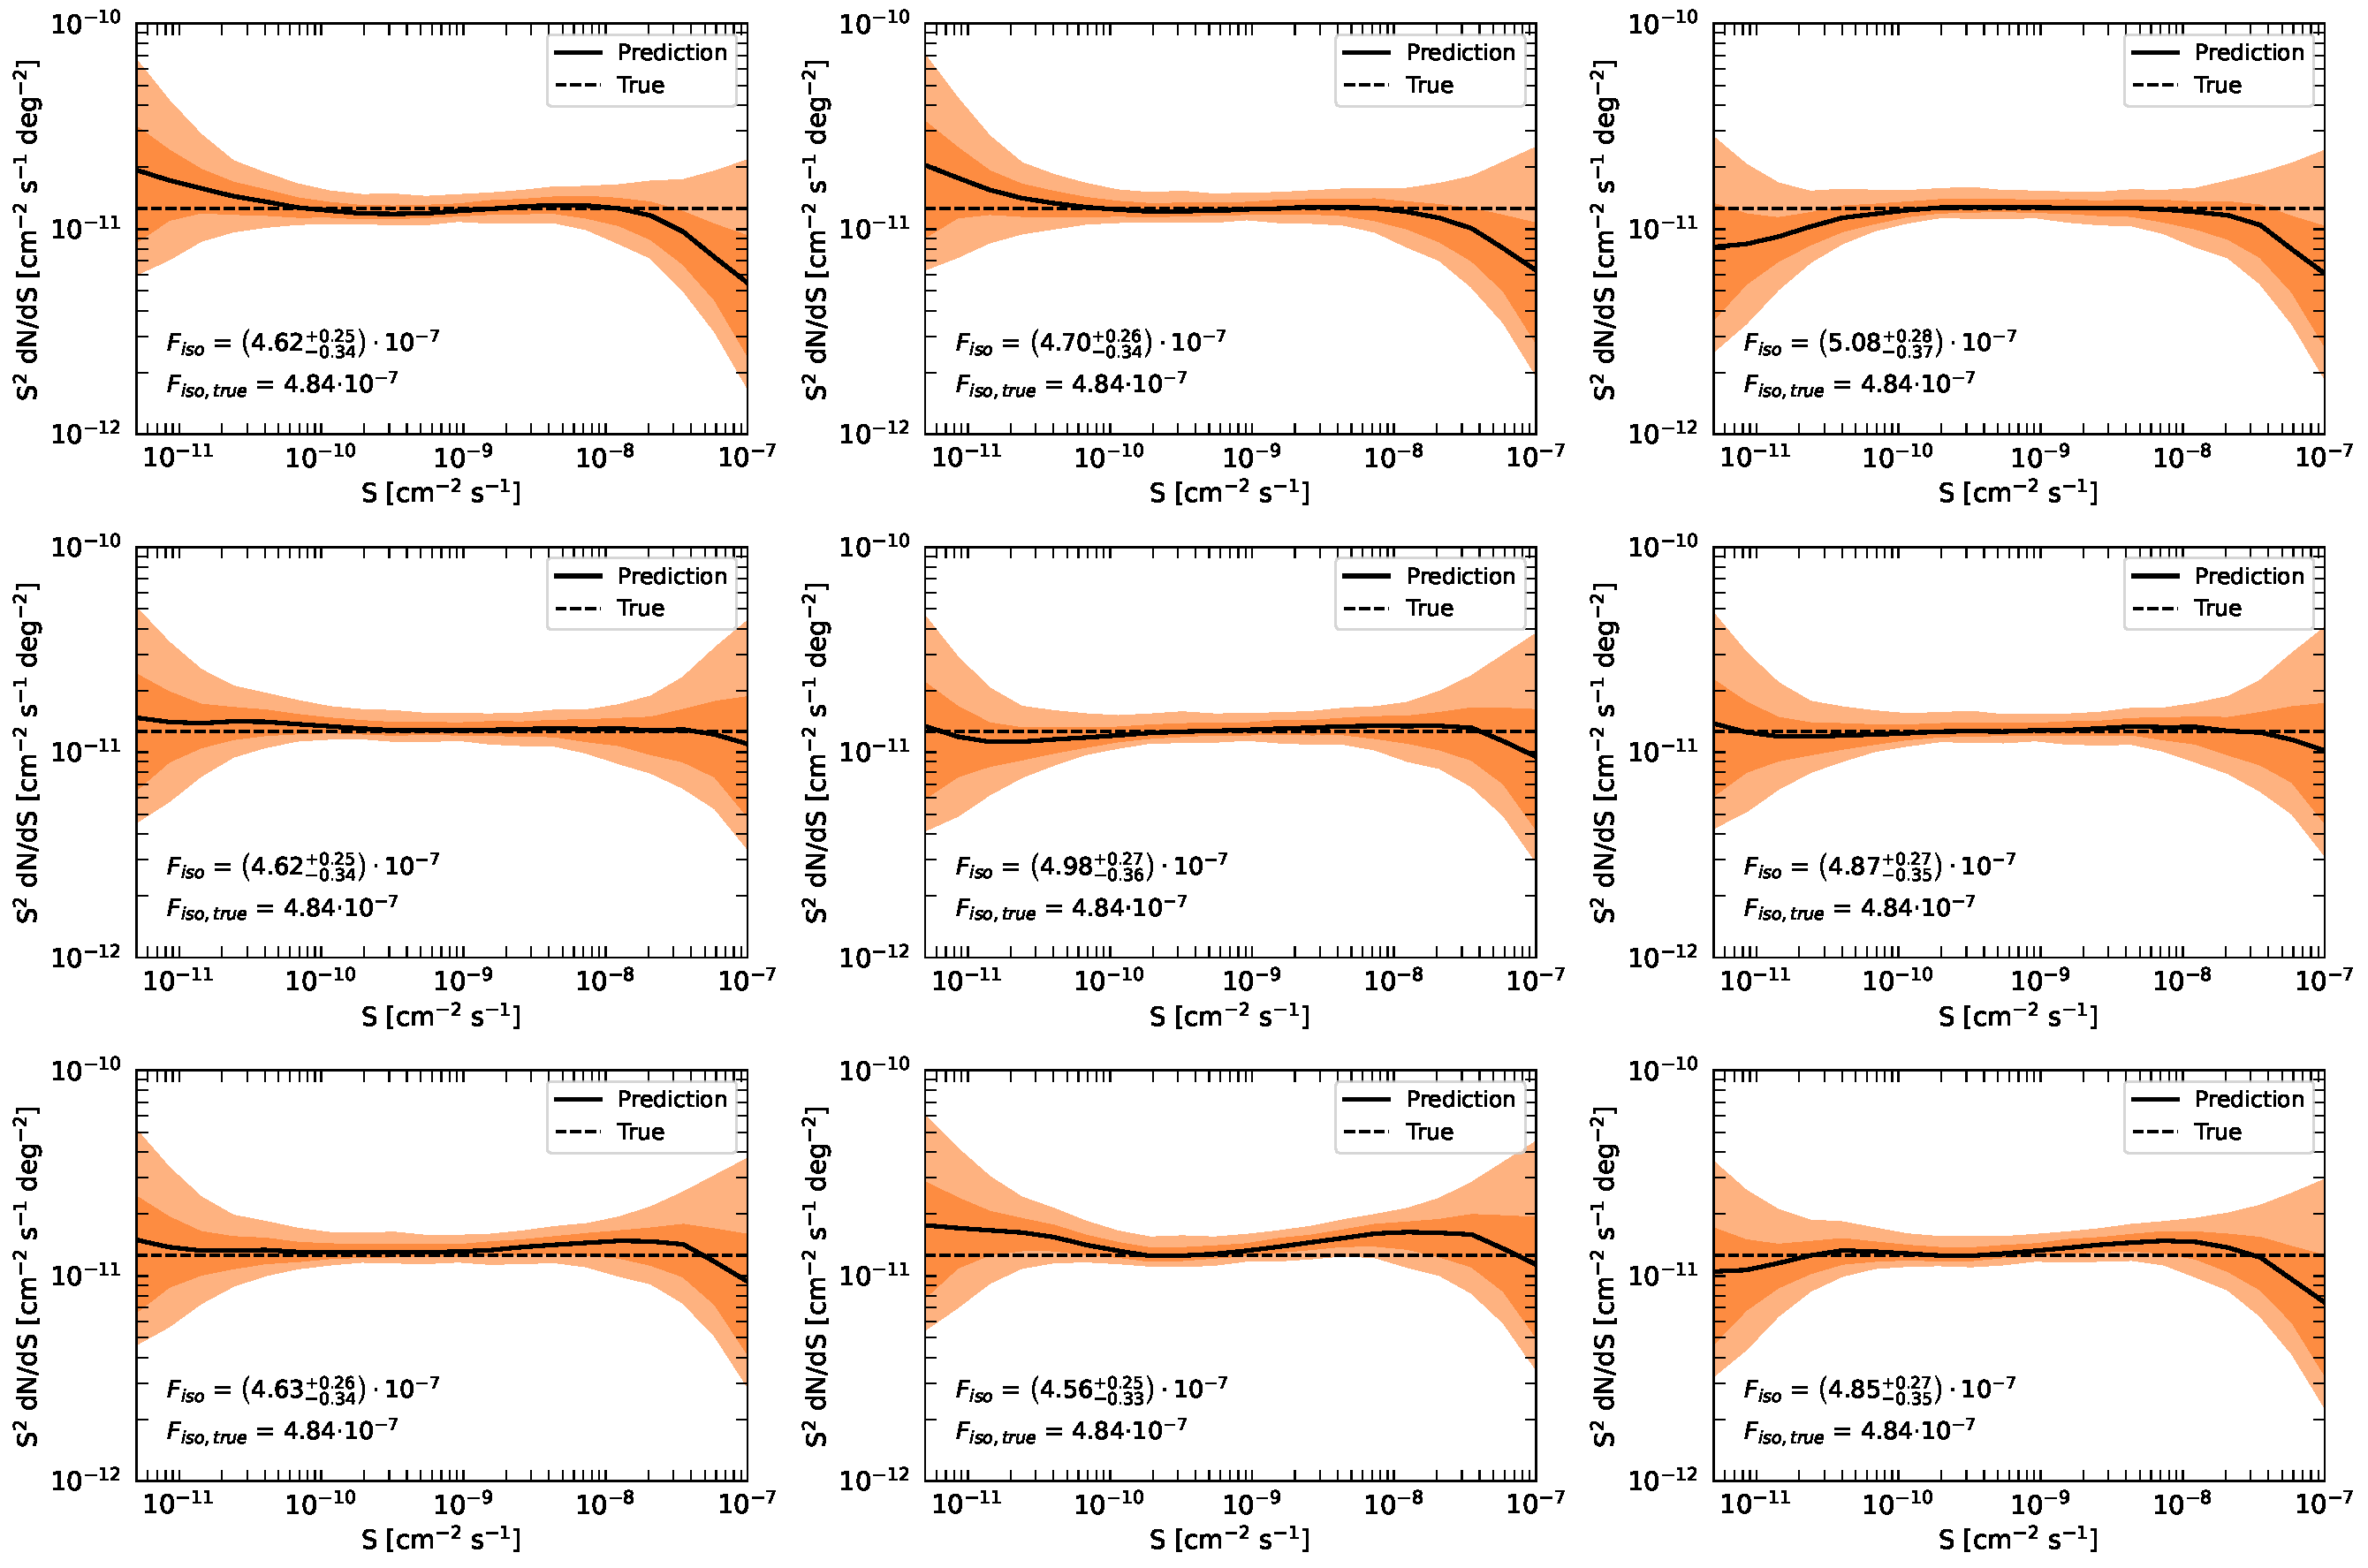
\includegraphics[width=1.0\textwidth]{chapter_06/sections/paper_dnds/img/model_plots/model_42/spherical/pendenza2.pdf}
\caption{Same as Figure \ref{fig:SphericalNN-test-random}  but for 6 different random realization of a flat $S^2\dnds$ and same 
$F_\textrm{iso}$.}
%$F_\textrm{iso,true}=4.84 \cdot 10^{-7}$ cm$^{-2}$ s$^{-1}$ sr$^{-1}$.   }
\label{fig:SphericalNN-test-flat}
\end{figure}

